\documentclass[letterpaper,11.5pt]{scrartcl}
\usepackage{totcount}
% \documentclass[11pt]{report}
% \documentclass{report}
% \documentclass{book}
\usepackage[bookmarks, hidelinks]{hyperref}
\usepackage{amssymb,amsmath}
\usepackage[title]{appendix}
% \usepackage{fullpage}
\usepackage{tabulary}
\usepackage{tabularx}
\usepackage{float}
% \usepackage[margin=0.50in]{geometry}
\usepackage[margin=1.00in]{geometry}
\usepackage[modulo]{lineno}
\linenumbers

\usepackage{booktabs}
\usepackage{pslatex}
\usepackage{apacite}
\usepackage{caption}
\usepackage{subcaption}
\usepackage{wrapfig}
\usepackage[english]{babel}
\usepackage{lmodern}
\usepackage{setspace}
\doublespace
% \usepackage{url}
\usepackage{bigfoot}
\usepackage[export]{adjustbox}
\setlength\intextsep{0pt}

% Colored comments 
\usepackage{color}
\definecolor{myorange}{RGB}{240, 96, 0}
\newcommand{\mt}[1]{{\textcolor{myorange} {({\tiny MT:} #1)}}}

\definecolor{myblue}{RGB}{30,144,255}
\newcommand{\jhj}[1]{{\textcolor{myblue} {({\tiny JHJ:} #1)}}}

\definecolor{mypurple}{RGB}{148,0,211}
\newcommand{\cm}[1]{{\textcolor{mypurple} {({\tiny CM:} #1)}}}

\definecolor{mygreen}{RGB}{26, 153, 51}
\newcommand{\ps}[1]{{\textcolor{mygreen} {({\tiny PS:} #1)}}}

\newtotcounter{citnum} %From the package documentation
\def\oldbibitem{} \let\oldbibitem=\bibitem
\def\bibitem{\stepcounter{citnum}\oldbibitem}

\usepackage{graphicx}
\usepackage{comment}

%\title{The form of uncertainty affects selection for social learning}
\title{Different forms of uncertainty differently affect the evolution of social learning}

\author{{}}

\begin{document}
\maketitle

\newcommand{\pisub}[1]{\pi_{\mathrm{#1}}}
\newcommand{\pilow}{\pisub{low}}
\newcommand{\pihigh}{\pisub{high}}
\newcommand{\piI}{\langle \pisub{I} \rangle}
\newcommand{\piS}{\langle \pisub{S} \rangle}
\newcommand{\ledger}{\bar\pi_{ib}}

\newcommand{\meanvar}[1]{\langle #1 \rangle}
\newcommand{\meansl}{\meanvar{s}}
\newcommand{\meanpi}{\meanvar{\pi}}
\newcommand{\meansoc}{\meanvar{\pi_\mathrm{S}}}
\newcommand{\meanasoc}{\meanvar{\pi_\mathrm{A}}}
\newcommand{\meanT}{\meanvar{T}}
\newcommand{\meanG}{\meanvar{G}}

\newcommand{\bandit}{\text{Bandit}_b(0, 1)}

\begin{abstract} 
  Social learning is essential to human survival---it is a critical
  adaptation for dealing with uncertainty. However, uncertainty takes many forms.
  We identified four theoretically important types of uncertainty: temporal
  environmental variability, ambiguous payoffs, decision set size, and effective
  lifespans. We used this framework to study conditions for the evolution of
  social learning in populations with cognitively realistic individual learning
  capacities.  We used evolutionary agent-based modeling to track how often social
  learning evolved. Agents performed one of several behaviors to acquire payoffs.
  Individual learning used the softmax algorithm. Social learning occurs between
  generations  through vertical and oblique transmission.  Different types of
  uncertainty had different effects. Temporal environmental variability suppressed
  social learning. Larger decision set sizes promoted social learning even
  when environmental change was more likely than not. Payoff
  ambiguity and lifespan had more complex effects on social learning, dependent on
  other uncertainty parameters.  This shows the importance of clearly
  operationalizing uncertainty in theories of social learning evolution.
% Social learning is essential to human survival. It is likely to evolve when it is more
% efficient than asocial, trial-and-error learning. Theoretically, social learning
% is adaptive for some uncertainty, but too much uncertainty makes
% social information unreliable. This fact is empirically
% supported across biology and human sciences. However, it is unclear how
% specific classes and types of uncertainty affect social
% learning evolution. Furthermore, existing models and experimental operationalizations of
% uncertainty are ambiguously related, and 
% tend to only consider a small number of behavioral
% choices.  Here we use evolutionary agent-based modeling to consolidate
% models of uncertainty in social learning evolution to address these issues.
% We model societies of agents who perform one of a number
% of possible behaviors to acquire payoffs in a time-varying environment.
% We identified complex patterns in social learning evolution depending on contextual
% uncertainty variables: environmental variability, ambiguous payoffs, 
% decision sets size, and effective lifespans. 
% Our work advances social learning evolution theory in a way that could help 
% guide human, non-human, and artificial intelligence towards optimal responses 
% to existential threats and new opportunities.
\footnote{This document contains
\total{citnum} references.}  
\end{abstract}


\section{Introduction}

Social learning enhances problem solving when acquiring information from others is more
efficient than learning on one's own~\cite{Laland2004}. However, social learning can also
lead individuals astray if, for example, they are copying outdated information.
Theoretical models have helped clarify the circumstances under which social learning
should be evolutionarily favored ~\cite{BoydRicherson1985}. This theoretical work has
motivated much empirical research and helped predict social learning behavior in humans
and other species ~\cite{McElreath2005,Kendal2018,Allen2019}.  This literature
demonstrates that social learning is a critical adaptation found across taxa for dealing
with uncertainty.  Uncertainty weighs particularly heavily on human adaptation because of
our long lifespans, cosmopolitan distribution, and the resulting necessity to adapt to
relatively coarse-grain environments \cite{levins1962}. However, the term ``uncertainty"
often conflates several different interpretations of that word. For example, different
models define uncertainty in terms of the rate of environmental change, spatial
environmental variation, or the reliability of information acquired from the environment.
Furthermore, in translating mathematical models to verbal predictions, the formal meaning
of terms like uncertainty is often lost \cite{lawson1988probability}, facilitating such
conflation. Furthermore, it can be important to distinguish a narrower definition of
uncertainty wherein the probabilities of outcomes remain unknown~\cite{knight1921,
volz2012}. As the number of formal models of social learning have expanded, an ever
increasing number of modeling choices ~\cite[Figure 1]{Kendal2018} and formalizations of
uncertainty have made it difficult to compare across models and consolidate our
understanding of the contexts in which social learning is adaptive. 
% Finally, while risk and uncertainty are often used interchangeably to refer to
% non-deterministic outcomes, 

Other (asocial) forms of learning may also be adaptations to uncertainty that could be
accounted for, but are typically glossed over.  In general, learning is an iterative
process by which one repeatedly acquires information, forms representations and
predictions, and tests and refines those representations and predictions to manage
uncertainty~\cite{jacobs2011bayesian,clark2013whatever}.  Because cultural evolutionary
models are more often used to explain social learning mechanisms, they tend to use a
single, weak individual-learning mechanism for comparison. Abstracting away asocial forms
of learning may lead us to underestimate the extent to which individual learning provides
quality information for social learning and for the individual to adapt to the challenges
assumed to be solved by social learning. 
% underestimate the quality of information
% available for social learning. 

To address these concerns we developed an evolutionary agent-based model that
simultaneously operationalizes several different forms of uncertainty and endows agents
with a relatively powerful learning mechanism. We have chosen to model four kinds of
uncertainty that are common in cultural evolution models and the related empirical
literature:  (1) temporal environmental variability; (2) selection set size (the number of
possible behaviors); (3) payoff ambiguity (the difference in the expected rewards for
different behaviors); and (4) the effective lifespan of agents (the number of
opportunities for individual learning), explained below. The model also assumes a more
cognitively realistic and empirically-motivated learning mechanism, the softmax algorithm.
This allows for a more accurate assessment of tradeoffs between 
social and asocial learning
by fleshing out an individual-level learning mechanism that makes full use of 
the individually and socially learned data. 
In this work, social learners learn from the previous generation, and 
asocial learners do not. All agents engage in individual-level learning within
their lifespans whether they are social learners or not.
We use this integrated model to ask what kinds of uncertainty are likely to
favor social learning, and to clarify the logic of why this would be the case.  

In the remainder of this introduction we describe previous research on the forms of uncertainty and the learning mechanism we include in our model. We then present how our evolutionary agent-based model works. Finally, we explain the logic underlying the result that different forms of uncertainty can either suppress or encourage the evolution of social learning. 

%% \cm{from Jamie's intro, not sure we should incorporate the rest here since our model doesn't speak much to things like heavy tailed distributions or adaptive toolkit work: Despite the technical difficulties of dealing with uncertainty, addressing it is an essential task because it potentially changes our understanding of decision-making in a qualitative manner. The dominant approach to understanding decisions for choices with variable outcomes is expected utility theory (EUT). As the name suggests, EUT requires the ability to calculate expectations, which means that we must know the probability distributions of outcomes. The non-probabilistic nature of uncertainty means one cannot calculate expectations. Following \cite{savage1954}, various research traditions in decision theory and economics have treated uncertainty as if it were risk, just with subjective probabilities replacing objective ones. The fundamental problem with this approach was noted by \cite{geweke2001} and further developed by \cite{weitzman2009}. In particular, the probability density function of an outcome that needs to be learned, but for which opportunities for learning are highly constrained, will be heavy-tailed and expected-utility calculations will not work because of the resulting undefined mass-generating function. Uncertainty implies heavy-tailed probability distributions and heavy-tailed distributions require different analytical methods \cite{nair_etal2022}....para...The heuristic-based adaptive-toolbox approach of \cite{todd_gigerenzer2000} provides an alternative strategy for understanding decision-making under uncertainty. There is a strong intuition that uncertainty should activate specific social-learning heuristics. Within the cultural-evolution literature, uncertainty is generally thought to lead to a social heuristic known as \emph{conformist-biased learning} \cite{boyd_richerson1985, henrich_boyd1998, muthukrishna_etal2016}....para...True uncertainty arises when an organism lacks the capacity to learn about the possible outcomes of a decision task. This is very likely for a cosmopolitan species living in a coarse-grain environment. Task complexity also. Non-stationary environmental change \cite{kay_king2020}. These potential sources of uncertainty can also interact.}




% \cm{I moved this for now: \emph{"Furthermore, many models of social learning evolution do not account for individual-level cognition~\cite{Heyes2016}, though humans clearly have evolved cognitive mechanisms for dealing with uncertainty generally~\cite{Gershman2019,Schulz2019}."} because I think it interrupted the flow and didn't seem directly linked to the goal of understanding aspects of uncertainty. However, if this is one of the main features of the model that we want to highlight as an improvement over previous work, then we probably have to say something more about it. Perhaps I just wasn't seeing the connection though, and the more accurate cognitive model DOES add to our ability to study the consequences of uncertainty. If that's the case, the argument should be sharpened. If not, maybe we put this info when the cognitive model is introduced.}\mt{Agreed. I put a first draft of a better version of this paragraph closer to/at the end of the Intro.}


%\mt{This paragraph is a first try to introduce the four uncertainty dimensions with examples to illustrate the problem we are answering. I outlined the next paragraph to get into more details of social learning: how cultural evolution works; conformity, success-biased, etc. Cristina, please edit this.} 

\subsection{Varieties of Uncertainty}

Uncertainty involves a reduced ability to predict what will happen in the future or to assess which actions are likely to yield particular outcomes. Uncertainty can manifest in many ways. We focus on the following four sources of uncertainty for the evolution of social learning: (1) temporal environmental variability, (2) selection set size, (3) payoff ambiguity, and (4) effective lifespan.

\textbf{Temporal environmental variability.} When external or internal shocks
(e.g., climatic events, migration, technological paradigm shifts) occur,
strategies that were previously adaptive may no longer be optimal. The difficulty
in predicting either when such shocks will occur or what behaviors will be
adaptive in the resulting environments leads to uncertainty. 

Temporal environmental variability is fundamental to most evolutionary models of
social learning. Such fluctuations have been proposed as an important selective
pressure for learned as opposed to genetically fixed behaviors
~\cite{Richerson2000}. On the other hand, environments that change too quickly
will lead the population away from social learning to avoid outdated, 
and therefore maladaptive information~\cite{Feldman1996,
BoydRicherson1985}. This suggests that intermediate levels of temporal variation
are important for the evolution of social learning mechanisms~\cite{aoki2005}.

Despite the theoretical centrality of temporal environmental variability, this construct is
implemented in several ways~\cite{aoki2014evolution}. Most commonly, it is modeled
as an independent probability of the environment changing its state each
generation
~\cite{BoydRicherson1985,Rogers1988,Feldman1996,McElreath2005,Enquist2007,perreault2012bayesian,aoki2014evolution}.
% The probabilities of environmental change are usually fixed per generation
% ~\cite{BoydRicherson1985,Rogers1988,kendal2009evolution}, 
but has also been modeled as deterministic cycles~\cite{Feldman1996, aoki2014evolution}.
Furthermore, the consequences of environmental change can range from mild to
catastrophic. In the latter case, a change of environment results in the total
elimination of any adaptive behavior, which must be learned \emph{de novo} for the
new environment~\cite{Rogers1988}. Such catastrophic environmental changes present
a large adaptive challenge as individuals cannot rely on accumulated information
from previous generations. Other models of environmental change introduce less
uncertainty as they fluctuate between two environmental states with corresponding
adaptive behaviors. This means that previously maladaptive
behaviors become adaptive when the environment changes
~\cite{perreault2012bayesian}. The chosen mechanism for modelling temporal
change has real theoretical consequences~\cite{aoki2014evolution}.


\textbf{Selection set size.}
When one does not know which option to take, uncertainty increases with the number of options, which we call the selection set size.
% This is a mathematical fact at the
% core of information theory: the number of bits required to reliably encode the optimal solution increases by one every time the
% selection set doubles in size~\cite{mackay2003information}. 
% This is intuitive; the more options to consider, the greater one's uncertainty about which option is the best choice. 
In studies of social learning, the selection set is often limited
to just two options.  For example, in empirical studies of \emph{bombus
terresteris} (bumble bee)~\cite{Baracchi2018} and \emph{parus major} (great
tit)~\cite{Aplin2017}, experimenters provided two behaviors for the bees or birds
to choose from, where one yielded a higher payoff than the other. %respectively,
each yielding greater or smaller payoffs depending on experimental treatment.
Similarly, many human studies have used just two or three possible
behaviors~\cite{McElreath2005,Toyokawa2019}. Behavioral study designs are
often motivated by modeling studies with similar formulations~\cite{Rogers1988,boyd1995does,
perreault2012bayesian}.
% \cm{pretty sure boyd1995 uses same trick as
% rogers 88 so not sure why they were being used as illustrating separate kinds of
% behavior selection sets. correct if wrong} 
Larger, more open sets of behavioral
choices are not uncommon in experiments trying to capture more complex or
naturalistic tasks~\cite{derex2013, wasielewski2014}, but these map on
imperfectly to the theoretical literature \mt{How so?}. Some models have studied systems with
larger, but defined, selection sets~\cite{Rendell2010}, while in others the
number of options is implicit in the model payoff structure
~\cite{Enquist2007} \mt{How does this work exactly in Enquist et al 2007?}. 
Researchers have also compared models with a different number
of environment states, corresponding to a different number of optimal behaviors
through time ~\cite{Feldman1996}. These examples share one common feature: 
the size of the selection set was held static \emph{within} model generations.
% as a measure of changing uncertainty in cultural evolutionary models.

\textbf{Payoff ambiguity.} Many models of social learning differentiate between
the payoffs for adopting optimal vs. non-optimal behaviors
\cite{Rogers1988,Enquist2007,Rendell2010}. The size of the difference between
these payoffs is usually taken to indicate the strength of selection of learning,
which makes sense. However, in reality payoffs for particular behaviors are not
always consistent. A behavior may yield a large payoff sometimes and a small
payoff other times \cite{McElreath2005}. This means that signals about the
relationship between behavior and payoff are often noisy, and differentiating
between behavioral options is in part a problem of signal detection.  When the
difference in expected payoffs between optimal and non-optimal behaviors is very
large, this noise matters little, as the signal is still very clear. However, when
the expected payoffs of different behaviors are similar relative to the size of
their variances, ambiguity arises about which behaviors really are superior.
Smaller differences between payoffs corresponds to larger ambiguity. Payoff
ambiguity has been manipulated in both theoretical ~\cite{perreault2012bayesian}
and empirical ~\cite{McElreath2005, Morgan2012} studies, both of which support the
claim that payoff ambiguity increases the reliance on social information.
Importantly, payoff ambiguity %differs from selection set size in that it not only
affects uncertainty, it also directly influences both uncertainty \emph{and} the
strength of selection. %This parameter sometimes takes the form of differences in
expected payoffs arising from different behaviors or
strategies~\cite{Enquist2007,Rendell2010} or by varying the standard deviation of
payoffs~\cite{McElreath2005}. 

\textbf{Effective lifespan.} 
The more opportunities one has for
learning in their lifespan, the more uncertainty can be reduced, assuming a
static environment. Similarly, a reduction in the number
of opportunities to learn will increase the uncertainty about whether one has
accurately learned about the available behavioral options and their associated
payoffs. That uncertainty is passed on to future generations.
% Learning is an iterative process by which one repeatedly acquires information, forms
% representations and predictions, and tests and refines those representations and
% predictions to manage uncertainty \cite{jacobs2011bayesian,clark2013whatever}. 
We refer to the number of learning opportunities as an individual's
effective lifespan to imply that it is the number of opportunities to learn
throughout the individual's lifespan that matters here, not necessarily how long
they live in the absence of relevant learning opportunities.  

Empirically, the number of learning opportunities can be manipulated in the lab,
but will also correspond with an individual's age the real world. In multi-round
studies of information use in novel tasks, US participants' use of social
information declined precipitously across rounds ~\cite{McElreath2005}, suggesting
they were more likely to use social information when they were most uncertain
about the task early on. In a more naturalistic context, Aplin et al. (2017)
\nocite{Aplin2017} found that younger great tits more readily used social
information compared with older individuals, possibly because they had accrued
less information via individual learning, and also possibly because younger
individuals have the most to gain (given their expected remaining lifespan) by
switching to superior behavioral options. 
% \ps{I got rid of the Leris and Reader reference because it didn't seem relevant
% to age-based uncertainty. They just showed that young guppies exposed to
% reliable models were more likely to use social information later. I also added
% some human studies, which seems important.} 
Cross-cultural studies on humans have shown the importance of childhood as a phase
of heavy social learning ~\cite{Reyes2016}. Young children are more likely to
acquire their beliefs and simple skills from their parents than are older children
or adults, which is at least partly due to the differential knowledge accrual
between young children and the older adults to whom they direct the most trust and
attention \cite{kline2013teaching}.
%The age of individuals was found to have an effect on social learning in both
%\emph{parus major}~\cite{Aplin2017} and \emph{poecilia reticulata}
%(guppies)~\cite{Leris2016}. \ps{What effect? I'm not sure } \mt{Need better
%connection between lifespan and age, or better references to support use of
%lifespan}.
The effective lifespan for learning
varies across tasks, individuals, and species, yet most models assume one learning
opportunity per generation ~\cite{Feldman1996,Henrich1998, perreault2012bayesian}.
Some models do allow several cultural generations within 1 genetic generation
~\cite{Enquist2007}, but little formal theory explicitly examines the role of
learning opportunities in social learning evolution models. 

%To answer our research questions about the combined effect of various forms of uncertainty on social learning evolution, we developed an agent-based model that incorporates all four of these uncertainty variables. We systematically vary these parameters to understand and predict their effects on social learning evolution.

% \subsection{Other adaptations to uncertainty} 
\subsection{Individual-level adaptations to uncertainty} 

% \begin{comment}

% \cm{I think a lot of this may be too much detail. I'm still editing and focusing the above on the main forms of uncertainty we are modeling and reviewing the relevant literature as we go. Yes we've made choices about things like horizontal vs vertical, but i think we can just justify that when we introduce the model }
% ps{I agree with Cristina here. I think we should use this section to justify our way of modeling individual and social learning, which is different from previous models. We don't need to provide a detailed review, just why it's worth doing it as we've done it. In particular, we should set up (1) social learning as an initial scaffold for future social learning, and (2) softmax individual learning which involves some greediness with occasional trial and error.}

% To add to confusion about how to integrate diverse models of social learning
% evolution, different models select different social learning components in
% seemingly \emph{ad hoc} ways 
% \begin{itemize}
%   \item 
%     Vertical, oblique, horizontal transmission
%   \item
%     Conformity, payoff-biased, frequency-dependent, etc. A note about how
%     ``conformity'' is often not distinguished from other forms of social learning
%   \item
%     Review human studies
%   \item
%     Review non-human studies~\cite{Leris2016,Aplin2017,Avargues-Weber2018,Baracchi2018}
%   \item
%     One sentence on how dual-inheritance theory enables us to gloss over whether
%     social learning is genetically or culturally evolved.
%   \item
%     More things from which we selected the operation of our model
% \end{itemize}

% \end{comment}

Social learning is the adaptive icing on the cake of other cognitive adaptations
to ecological uncertainty.  While the literature reviewed above suggests that
several forms of uncertainty play a role in favoring the evolution of social
learning, several other cognitive mechanisms have also evolved in response to
uncertainty ~\cite{volz2012}. Many of these are flexible learning mechanisms that
do not require assessing others' information. For example, people in experimental
studies increase their exploratory behavior when total uncertainty in the task
increases and are more likely to test %Furthermore, correlations in uncertainty
between potential behaviors, humans tend to adopt directed exploration strategies
that favor testing behaviors with greater observed payoff variance
\cite{Wilson2014,Gershman2019}.

Many models of social learning assume little to no cognitive capabilities
of their agents. For example, a common modelling strategy compare the payoffs of
agents with different pure learning strategies (some will always engage in social
learning, and others in individual learning) while revealing nothing about the
cognition underlying individuals' decisions  ~\cite{BoydRicherson1985, Rogers1988,
aoki2005}. Some more complicated learning strategies that make use of both
socially and individually learned information have been proposed
~\cite{Enquist2007, perreault2012bayesian}, but these are seldom designed to
reflect cognitive mechanisms for integrating information. Though such
simplifications are often useful, several authors have warned of the risks to
\emph{blackboxing}, or ignoring, cognitive mechanisms \cite[p. 658]{Heyes2016,
Kendal2018}, given such details may be theoretically meaningful. In order to
understand how social learning evolves as an adaptation to uncertainty, we need to
endow agents with a biologically plausible cognition capable of integrating
information from various sources in a payoff-maximizing way~\cite{Gershman2019}. 
% \cm{I don't
%   understand this next sentence, but think it can be cut with no loss of meaning:
%   In our model we do not impose any structure in randomness between behaviors, so
% our cognitive model is only sensitive to total randomness.} 
To do so, we let
agents see the payoffs to behaviors and use the softmax function to convert these
observations to a probability distribution from which they strategically select
their own behavior. %\cm{does this still make sense? and does it need a citation?}

%\paragraph{Meaning of uncertainty in ecology (and cognitive and social sciences?) } (JAMIE, PAUL?) \ps{I've added a bunch to the section on different types of uncertainty, which could be more fleshed out if we like. I don't think an additional section here is needed.}
%We need to support our claim that these four classes of uncertainty really count as forms of uncertainty and show how it is consistent across ecology, and maybe connect to uncertainty in cognitive and social sciences more broadly. 

%\paragraph{Evolutionary ABMs for social learning evolution theory development} (PAUL)
%\ps{I'm not sure a section is needed on this, but we can add something about how ABMs allow us to capture complexity not possible with purely mathematical approaches. I think it probably makes the most sense to address this at the beginning of the model description.}

\section{Model}

% \cm{Other choices we made that might need to be justified: 1) softmax: existing models underestimate the power of learning from experience by not having a rich cognition. This rich cognition can improve both individual learning and help social learners recover from outdated / misleading social info. 2) no conformism: but that's ok because we're giving social learning the best chance of success. 3) no horizontal transmission, no spatial variation}

To understand how uncertainty affects social learning, 
we developed an agent-based model of
social learning evolution.  Evolutionary agent-based models simulate changes in
prevalence of a phenotype over several generations---in this model the phenotype
is whether or not an agent engages in social learning.  In the model, a
population of $N$ individuals each must decide which of $B$ behaviors to perform at
each time step within a generation consisting of $L$ time steps. At the end of each
generation, agents are selected with replacement to reproduce another $N$ agents, 
biased by net payoffs. Agents
who inherit the social learning trait then learn about payoffs from the
previous generation, while asocial learners begin life with no \emph{a priori}
knowledge of the world.  Each behavior is a ``bandit'', a common modeling and
experimental approach for representing behaviors with Bernoulli-distributed
payoffs~\cite{SuttonBartoBook,McElreath2005,Steyvers2009,Rendell2010,Schulz2019}.
All bandits thus yield a payoff of 1 or 0 with a certain probability.  One of the
bandits/behaviors in the model is more likely to pay off than all the rest.  Agents
optimize their net payoffs over their lifespan by quickly figuring out which
behavior is optimal and performing it as often as possible within their lifespan.

We operationalized four separable varieties of uncertainty that affect the
ability of agents to find and choose the optimal behavior: 
\emph{environmental variability}; 
\emph{selection set size}; \emph{payoff ambiguity}; and the \emph{effective lifespan}. 
Environmental variability is the probability that the optimal behavior changes
between generations. We do not consider within-generation variability. 
Furthermore, our model is not spatial, so agents have free, instant
access to all behaviors, and there is no spatial uncertainty. 
These conditions reflect humans in a computer-based social learning evolution
experiment~\cite{McElreath2005,Morgan2012,Derex2016}. Spatial dimensions could also be
considered irrelevant if costs associated with accessing a behavior were equal,
e.g., if it was assumed to be equally costly for animals to
visit alternative food sources~\cite{Aplin2017,Baracchi2018}.  
% This is empirically justified since cultural evolution
% occurs when meta-cognitive strategies and information are transferred via
% learning and social influence, instead of by physical reproduction and death
% as in genetic evolution.  
The selection set size is the total number of possible
behaviors agents choose from, assumed to be constant within a simulation.  
Payoff ambiguity is the payoff difference between optimal
and non-optimal behaviors. The effective life span is the
number of time steps in which agents perform behaviors within a generation. 
Each simulated environment provides a distinct challenge
to the agents, which will lead agents to differently evolve to become social
learners or not, depending on which strategy optimizes net payoffs.

\emph{Agents} here are autonomous, intelligent, simulated problem solvers. Each
agent evaluates its environment and chooses how to act within that environment based
on a set of empirically-motivated rules.  Our agents select which behavior to do
probabilistically, weighted by the softmax function applied to the mean payoff they
have observed for each behavior. The softmax function is a biologically plausible
generalization of behavior selection under uncertainty that enables agents to often
greedily exploit the most lucrative behavior (based on their observations) but also
to sometimes explore alternatives~\cite{Schulz2019,Collins2013,Daw2006,Yechiam2005}.
Such individual-level intelligence is a critical adaptation that has apparently
co-evolved with the capacity for social learning, and has a marked influence on the
cultural evolution of social learning as we will demonstrate in our Analysis.
We will see that individual-level intelligence allows agents to recover from
the receipt of outdated information due to temporal environmental variability.

In \emph{evolutionary} agent-based models like ours, agent life cycles are
programmed to cause agents to reproduce and die off, where reproducers pass on
heritable traits to their offspring. 
Natural selection occurs in the model when agents with higher
payoffs preferentially reproduce. This is a model of cultural evolution, so
``reproduction'' means teaching the meta-cognitive strategy of whether one should learn
socially at all; ``death'', in this interpretation, means
loss of the potential to socially influence others. 
This sets up an inter-generational structure
that we also use as a scaffold for social learning: we assume social learning occurs
\emph{obliquely}, meaning learning happens when a new
generation of agents each select a teacher from the previous generation, possibly
including their parents.  
Evolution, then, acts as an optimization routine to identify which heritable trait
values are most rewarded under in different environmental uncertainty contexts,
defined by different uncertainty parameter settings
(Table~\ref{tab:uncertaintyParameters}).  

Agents have one heritable trait in this model, whether or not
an agent, $i$, learns socially, denoted $s_i$. $s_i$ is binary: it is 1
if the agent is a social learner, and 0 otherwise. In our analysis, we 
aggregate $s_i$ over all agents and simulation trials to understand the affects of
different uncertainty parameter settings. 
Our computational analysis amounts to observing patterns in
the aggregated $s_i$, supported by measuring the number of generations 
to model convergence and expected payoffs. 
To understand how different varieties of uncertainty interact
to affect the evolution of social learning, we systematically created an array of
simulated environments by systematically varying the uncertainty parameters. 


\subsection{Model environment and uncertainty}

The model environment provides behaviors for agents to perform. The structure
of the environment is specified by setting several parameters, including
three of the uncertainty parameters: environmental variability, selection set size, 
and payoff ambiguity. 
Each behavior is indexed by $b$ and modeled as a ``one-armed bandit'', which yields 
Bernoulli-distributed payoffs of 1 with probability $\pi_b$ and 0 with 
probability $1 - \pi_b$. $\pi_b$ is equivalently the expected
payoff of behavior/bandit $b$. The model environment affords $B$ behaviors, where
$B$ is the \emph{selection set size} uncertainty parameter, which
is constant throughout the course of a given simulation, but varied systematically
across simulations. 

The model environment is dynamic: which behavior is optimal changes between
generations with probability equal to the \emph{environmental variability}, $u$.
At the beginning of each generation, one bandit is optimal and yields expected
payoff $\pihigh$; the other $B-1$ behaviors yield a lower payoff, $\pilow$. 
The \emph{payoff ambiguity} is defined by $\pihigh - \pilow$. 
We set $\pihigh = 0.9$, constant across all simulations, so we vary
payoff ambiguity by varying $\pilow$, i.e., payoff ambiguity increases with
$\pilow$.  


\vspace{2em}
\begin{table}[h]
\caption{Model ecological parameters, including uncertainty parameters $u$, $B$,
$\pilow$, and $L$. Bold indicates default value tested} %\emph{default value tested}.}
    \label{tab:uncertaintyParameters}
    \centering %\hspace{-3em}
    \begin{tabular}{cp{4.0in}p{1.25in}} \toprule

        Symbol & Description & Values tested \\ 

        \midrule  

        $u$    & Probability optimal behavior changes between generations 
               & 0.0, 0.1, \ldots, 1.0 \\

        $B$       & Number of ``bandits'', i.e., behavior options
                  & 2, 4, 10 \\

        $\pihigh$ & Probability that the unique optimal behavior pays off 1 
                & \textbf{0.9} \\

        $\pilow$ & Probability one of $B - 1$ non-optimal behaviors pays off 1 
                 & 0.1, 0.45, 0.8 \\ 

        $L$    & Time steps per generation & 1, $B/2$, $B$, $2B$, $4B$ \\

        $N$    & Population size
                 & 50, 100, 200, \textbf{1000} \\
               
        \bottomrule
        \end{tabular} 
\end{table}



\subsection{Agents and learning}

Agents are endowed with dynamic attributes to intelligently select behaviors and
calculate average payoffs for each behavior. All agents engage in
individual learning over their lifespan, whether or not they are social learners.
Social learners begin life with
behavioral preferences based on information from their
teacher, an agent from the previous generation. 
Asocial learners begin life with no behavioral
preferences. 
% Agents and their learning procedures are specified through several
% parameters introduced below.


\subsubsection{Individual learning}

All agents perform individual, trial-and-error learning at each time step in
their lifespan.  Learning is guided by softmax search. Softmax search
guides agents to more frequently exploit the most profitable behaviors when the
agent is more certain which is optimal, and to explore more frequently when the
agent is unsure.  To do softmax searching, agents track average payoffs acquired
from each behavior, which also requires agents to track the number of times they
have performed each behavior.  We denote the average payoffs obtained by agent $i$
for behavior $b$ as $\ledger$. We denote the number of times $i$ performed $b$
as $c_{ib}$ (``$c$'' stands for count). 
At each time step, agents perform behavior $b$ with softmax-weighted probability
\begin{equation}
  \Pr(\text{Agent $i$ performs behavior $b$}) = 
    \frac{e^{\beta \ledger}}{\sum_{b=1}^B e^{\beta \ledger}}.
\end{equation}
\noindent
$\beta$ adjusts how frequently agents perform 
behaviors with high expected payoffs (larger $\beta$) versus how frequently
agents explore alternative behaviors (smaller $\beta$)~\cite{McElreath2005}. 


\subsubsection{Social learning}

At the beginning of each generation other than the first, social child agents select
one member of the previous generation to learn from, if the child inherited
$s_i = 1$. A child agent $c$ is a social learner if its parent $p$ was a social
learner, i.e.\ $s_c \leftarrow s_p$, without mutation.  Social learner children
select a teacher from the previous generation by first selecting $N_T$ prospective
teachers fully at random, then by sampling from the $N_T$ with each prospective
teacher weighted by their net payoffs relative to the other $N_T - 1$.


\subsubsection{Social learning as a scaffold for individual learning}

In this model, being a social learner is beneficial when it is more likely on
average to provide greater net payoffs than being an individual learner.  It is not
catastrophic for an individual to receive outdated information, as is sometimes
assumed~\cite[e.g.]{Rogers1988}. Instead, agents explore alternatives and
greedily perform different behaviors that pay off better. 
This mechanism is critical for explaining the patterns we observe in the 
Analysis, where social learning evolves when $u > 0.5$.
In this case, the optimal behavior will switch between generations more often than
not. Without individual learning, social learning would not evolve when $u > 0.5$.

\begin{table}[h]
  \vspace{2em}
  \caption{Agent-level variables. The first four ($\protect s_i$, $\protect
    \bar\pi_{ib}$, $\protect c_{ib}$,
  and $\protect \pi_i$) are dynamic with an implicit time dependence. The softmax
greediness $\protect \beta$ and number of prospective teachers for social learners,
$\protect N_T$, are constant throughout each simulation.}
    \label{tab:modelParameters}
    \centering %\hspace{-3em}
    \begin{tabular}{cp{4.0in}p{1.25in}} \toprule

        Attribute & Description & Initial value \\ 

        \midrule  

        $s_i$  & Social learner trait: 1 if agent $i$ is social learner; 0 otherwise & 0
        or 1 equally likely \\

        $\bar\pi_{ib}$ & ``Ledger'': mean payoffs acquired via behavior $b$ by $i$ 
                       & $B$-vector of zeros \\

        $c_{ib}$ & Count of how many times agent $i$ performed $b$ 
              & $B$-vector of zeros \\

        $\pi_i$ & Net payoffs accumulated by $i$ within generation & 0.0 \\

        $\beta$ & Softmax greediness; $\uparrow=$more exploitation, $\downarrow=$more
                    exploration 
               & 1, \textbf{10}, 100 \\
        
        $N_T$    & Number of teachers to pool, from which best selected 
                 & 2, \textbf{5}, 10, 20  \\

        \bottomrule
    \end{tabular}
\end{table}



\subsection{Dynamics}

Model dynamics proceed by first initializing the environment and agents according
to parameter settings for the simulation. Then, within each generation,
agents select and perform behaviors, updating their observations along the way.
Between generations, agents reproduce, teach child agents, and die off. 
Child agents then begin a new round of generational dynamics, followed by
reproduction. This process continues until the population has fixated as
all social learners or all asocial learners, or until an upper limit of 
iterations has been reached. This process is visualized in
Figure~\ref{fig:schematic}.


\paragraph{Initialization}

The model is initialized with $N$ agents, all with zero observed mean payoffs, 
$\ledger = 0$, and zero counts of how many times
they have tried each behavior, $c_{ib} = 0$ (Figure~\ref{fig:schematic}A).
At generation start, one of the behaviors is set to 
yield expected payoff $\pihigh$, with the other $B-1$ behaviors yielding
expected payoffs $\pilow$. Agents are independently randomly initialized with $s_i
\in 0,1$.


\paragraph{Within-generation dynamics}
% To guide behavior selection, agent $i$ counts how many times it
% performed each behavior $b$, denoted $c_{ib}$. Agents use this count to 
% update the mean payoff they have obtained from behavior $b$, denoted $\ledger$.
% $\ledger$ is initialized to 0 for all $b$ at model start for
% all agents (Figure~\ref{fig:schematic}A), and at 
% generation start for asocial learners. Social
% learning agents' $\ledger$ is initialized as that of its teacher, who is selected
% through performance-biased oblique learning; $c_ib$ is set to 1 for all social
% learners $i$ and behaviors $b$ (Figure~\ref{fig:schematic}C). Agent $i$'s
% accumulated payoffs from performing several behaviors over their lifetime of $L$
% time steps is denoted $\pi_{i}$. If an agent $i$ is a social learner, then we write
% $s_i = 1$, otherwise the agent is an asocial learner and $s_i = 0$.

Within each generation, all $N$ agents perform $L$ behaviors sequentially and
independently (Figure~\ref{fig:schematic}B).
Agents make one choice for each step in its lifespan using softmax weighting
described above, updating the mean payoffs it has observed along the way. 
Agents probabilistically recieve a payoff of 0 or 1 depending on whether the
bandit paid off. Behavior payoffs are drawn from a 
Bernoulli distribution with mean $\pi_b$, so $\pi_b$ is also the mean payoff from
behavior $b$.  For concreteness we denote this probabilistic payoff
$\bandit$. After performing behavior $b$, agent $i$ updates the
corresponding \emph{behavior count} by 1, $c_{ib} \leftarrow c_{ib} + 1$, and then
the expected payoffs calculated for that behavior are updated with
exponentially-weighted averaging
\begin{equation}
  \ledger \leftarrow \ledger + \frac{\bandit - \ledger}{c_{ib}}.
\end{equation}
\noindent


\paragraph{Intergenerational dynamics}
Between generations, agents first reproduce via asexual haploid reproduction; 
then new child agents learn from the
previous generation if they are social learners; and finally all agents from the
previous generation then die off (Figure~\ref{fig:schematic}C). 
$N$ reproducers are selected with replacement over $N$ independent draws, 
biased by performance:
\begin{equation}
  \Pr(\text{Agent $i$ is chosen to reproduce in one draw}) = \frac{\pi_i}{\sum_{i=1}^N \pi_i}.
\end{equation}
\noindent
A child inherits its parent's social learning trait $s_i$ without mutation.
A social learner child with $s_i = 1$ learns from a teacher from its parent's
generation, including possibly their parent (oblique learning). 
A child selects its teacher by first selecting $N_T$ prospective
teachers from the population completely at random, then selecting the one with
highest net payoffs $\pi_i$ as their teacher, with ties broken randomly. While it
is somewhat arbitrary to first subset $N_T$, this is a conservative choice that
represnts the fact that access to the entire population is not generally guaranteed.
Social learners adopt their chosen teacher's expected payoffs observations $\ledger$,
and set all $c_{ib} = 1$ so expected payoffs remain within $[0, 1]$.  Asocial
learners ($s_i = 0$) are initialized with $c_{ib} = 0$ and $\ledger = 0$ 
(Figure~\ref{fig:schematic}C). The
newly initialized population then repeats within-generation dynamics. 

After reproduction and die-off, the optimal behavior changes with probability
$u$. The new behavior is chosen from all other behaviors, with the 
current optimal behavior excluded from selection.

\paragraph{Stopping conditions} The evolutionary process continues until the
population reaches evolutionary fixation with repsect to social learning, where
$\sum_i s_i = 1$ or $\sum_i s_i = 0$, or until 20k iterations have run. 
It is rare for simulations not to reach fixation. We report how frequently
this happens in Table~\ref{tab:convergence}.

\clearpage

\begin{figure}
  \caption{Agents are randomly initialized as social learners or not, with their
  payoff observations all initialized to zero (A). Then agents begin selecting
and performing behaviors and accumulating payoffs, which goes on for $L$
timesteps (B). After $L$ time steps, agents are selected to reproduce,
social learner children learn from a member of their parent's generation, and
the previous generation dies off (C). The simulation stops if children are all
social or asocial learners (i.e.\ the system reaches fixation), 
otherwise repeat another generation and evolution (3).}
  \label{fig:schematic}
  \centering
    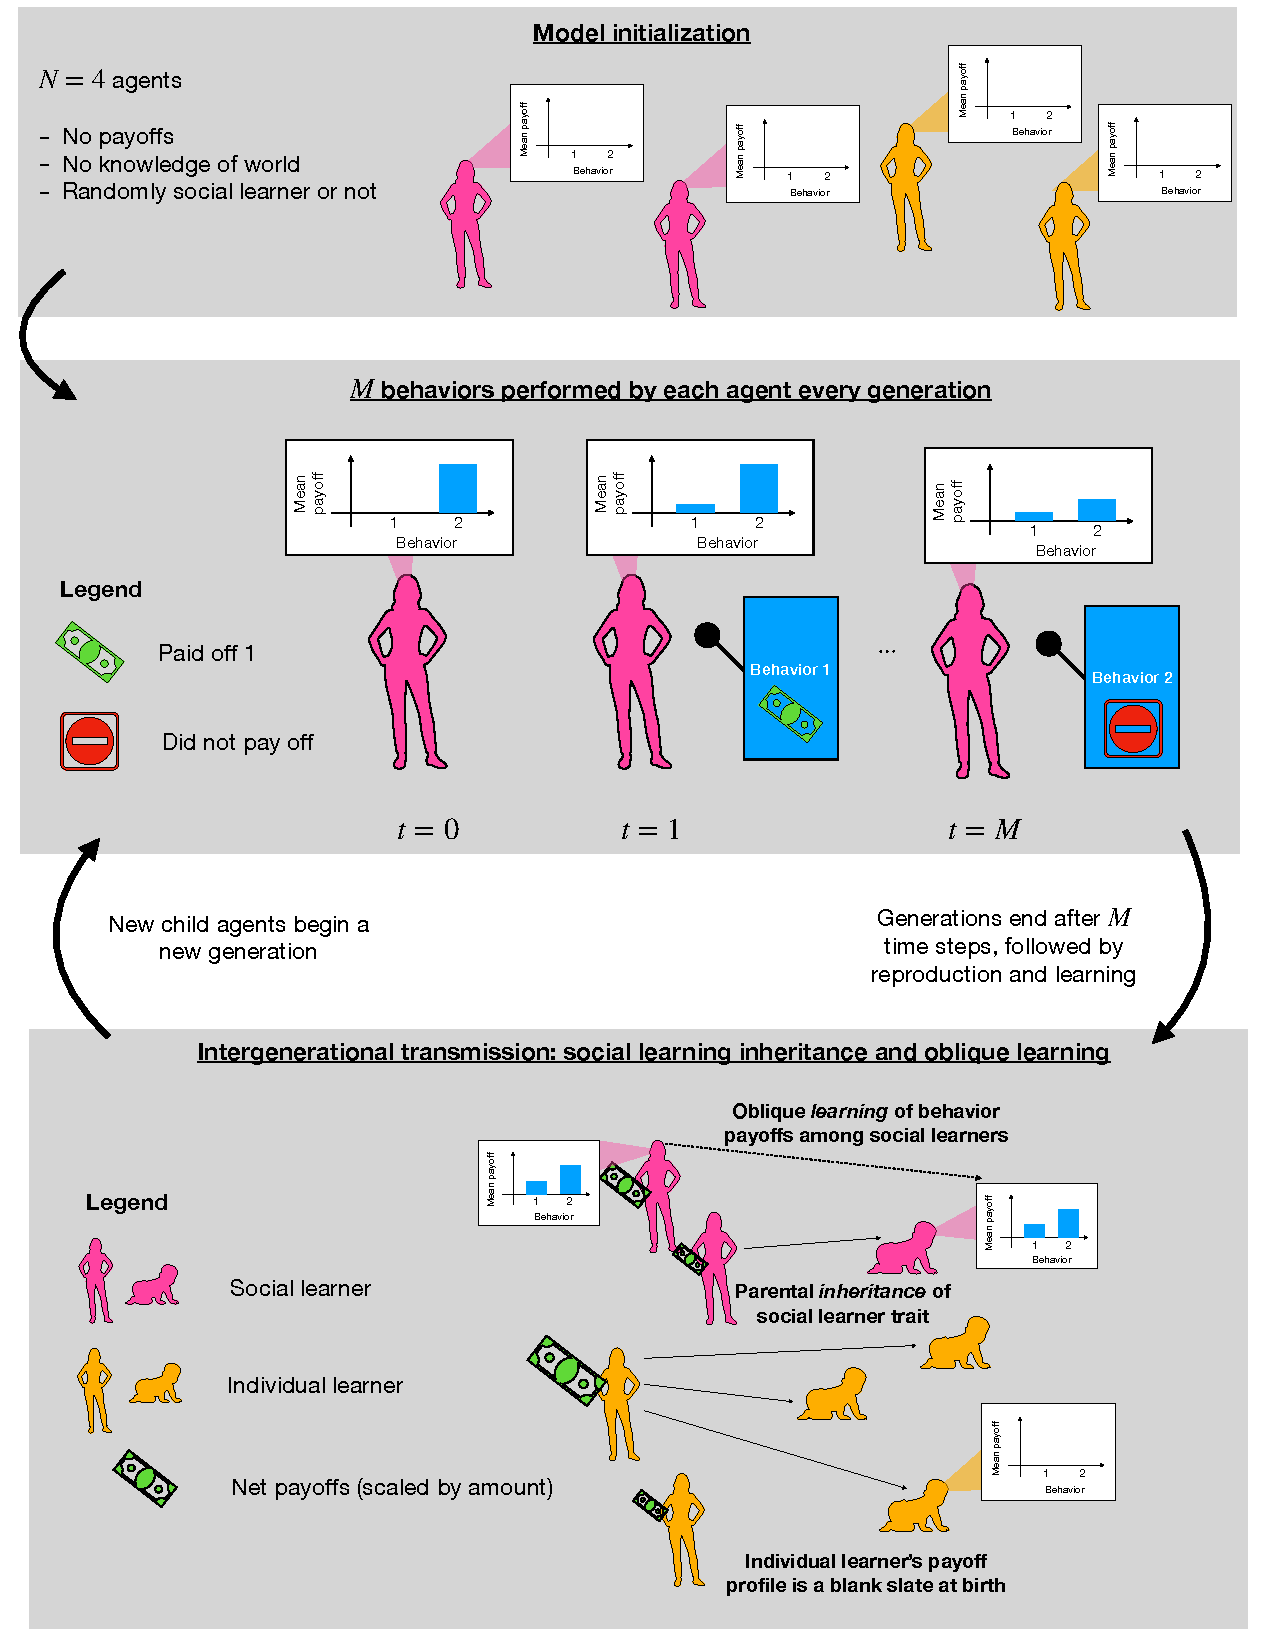
\includegraphics[width=\textwidth]{Figures/IntraInterGenerationalDynamics.pdf}
\end{figure}


\subsection{Computational analyses}
\label{ssec:computationalAnalyses}

% We developed a series of computational
% analyses of the effect of uncertainty on social learning evolution by 
% systematically varying uncertainty parameters and observing how
% frequently model populations evolve to be social learners.  

To analyze the effect of the four principal uncertainty factors, we systematically
varied uncertainty values and observed how frequently social learning evolved across
1000 trial simulations. We varied $u \in
\{0.0, 0.1, \ldots, 1.0\}$; $\pilow \in \{0.1, 0.45, 0.8\}$; $B \in \{2, 4, 10\}$;
and $L \in \{1,2,4,8\}$ for $B=2$ and $L \in \{1,B/2,B,2B\}$ for $B=4,10$.  We
observed three outcome measures, with $\meansl$ as the primary measure: 
the average value of $s_i$ over all agents and trials. To support our conclusions
based on $\meansl$, we also measured $\meanpi / L$, the average net 
payoffs at simulation end across agents and trials, normalized by lifespan; 
and $\meanG$, the mean
number of generations to fixation. We analyze outcomes by
plotting $\meansl$ on the y-axis and environmental variation is on x-axis since we
theoretically expect that $\meansl$ will decrease monotonically from 1 to 0 as $u$
increases. Note that the hypothesis-testing concept of significance is meaningless
here because we could make any small outcome difference ``significant'' by running
more simulation trials.  We instead study the patterns of outcome variables over
systematically varied uncertainty factor values. 

\begin{table}[h]
    \caption{Outcome variables.}
    \label{tab:outcomeVariables}
    \centering %\hspace{-3em}
    \begin{tabular}{cp{4.25in}p{0.85in}} \toprule

        Symbol & Description & Values \\ 

        \midrule  

        $\meansl$ & Mean social learning prevalence over agents and trials
                  & $\in [0.0, 1.0]$ \\

        $\meanpi / L$ & Mean payoffs accumulated in a generation normalized by
        lifespan & $\in [0.0, 1.0]$ \\

        $\meanG$ & Mean number of generations to convergence & 20k / 8 max. \\
        \bottomrule
    \end{tabular}
\end{table}

\subsubsection{Sensitivity analyses}

We performed sensitivity analyses to ensure that our main analysis is reasonably
robust to a range of auxiliary parameters. Specifically,
we varied the population size, $N$, to explore whether smaller $N$ would 
show more drift due to finite population size effects, but also generally support
our main conclusions. Next, we varied the
softmax greediness parameter $\beta \in \{1, 100\}$ to supplement the main results
that used $\beta = 10$. We do not
expect agents with different $\beta$ to perform equally well 
individually, so certain $\beta$ values may themselves suppress social learning
by undermining individual learning. Nonetheless, our results
should be valid over some range of $\beta$. Finally, we varied the
number of prospective teachers $N_T \in \{2, 10, 20\}$ 
to supplement the main results that used $N_T = 5$. The number of prospective
teachers should not change whether social learning is optimal, 
but it may induce more drift since the benefit of social learning may
be more difficult to detect with fewer prosopective teachers.


\subsubsection{Implementation}
Our model was implemented in the Julia programming language~\cite{Bezanson2017} 
using the Agents.jl agent-based modeling library~\cite{Datseris2022} and run
on the Sherlock supercomputing cluster at Stanford University. Model code and
data are publicly available on GitHub\footnote{\url{https://github.com/mt-digital/UncMod}}.


\section{Analysis}

To understand how different forms of uncertainty interact to affect the evolution of
social learning, we measured how frequently social learning evolved across
uncertainty parameters. We analyzed outcomes by plotting the mean observed social
learning frequency, $\meansl$, with mean taken across all agents and 1000 simulation trials for each
uncertainty parameter setting.   
% This is convenient because we are most certain about how $\meansl$ depends on $u$:
% we expect $\meansl$ to decrease as $u$ increases since environmental variability
% is well understood to cause socially-transmitted information to become outdated. 
% To inspect patterns in $\meansl$ over all uncertainty parameters, 
We analyze nine plots of how $\meansl$ (y-axis in each plot) changes over $u$ (x-axis) 
in a $3\times3$ plot array (Figure~\ref{fig:mainResults}). 
% All plots show how $\meansl$ changes (y-axis)
% with environmental variability, $u$ (x-axis). 
Selection set size, $B$ increases from left to right in the plot array (columns). 
Payoff ambiguity increases as $\pilow$ increases from top to bottom in the array 
(recall $\pihigh=0.9$ for all analyses).
Effective lifespan, $L$, is indicated by line and marker colors (inset). 
Several patterns in social learning prevalence emerged as 
these uncertainty parameters were varied (Figure~\ref{fig:mainResults}). 
% We support our conclusions regarding the evolution of social learning by analyzing
% the time to fixation and by comparing the average net payoffs in our simulations
% to the expected payoffs for individuals in both populations of all social learners
% and in populations of all individual learners. We thus use our analysis to
% understand changes to how $\meansl$ changes over $u$ for different uncertainty
% parameter settings.

First, we confirmed the current theoretical understanding that greater $u$ uniformly decreased
$\meansl$ across all other uncertainty parameter values. The other uncertainty
parameters changed the $u$ value at which $\meansl$ began to decrease,
and how rapidly $\meansl$ decreased over $u$. 
For example, when payoff ambiguity and selection set size were
both small ($\pilow = 0.1$ and $B=2$), social learning evolved only when $u$ was
small. 
% These parameter settings present a relatively easy problem for individuals.
% Furthermore, it is relatively costly for agents to be misled by outdated social 
% information in this case, especially for longer lifespans for finding the 
% optimal behavior (Figure~\ref{fig:mainResults}, upper left). 
When $\pilow = 0.8$ and $B=2$, for exapmle, $\meansl$ decreased less rapdily over $u$ due to 
drift caused by weak selection caused by little advantage for performing the optimal versus
non-optimal behavior (see rows of Figure~\ref{fig:mainResults}). We analyzed several
such patterns of social learning evolution and suppression across different uncertainty settings.

Increased selection set size $B$ led nearly uniformly to more prevalent social
learning, with all other uncertainty parameters held constant. This is first 
because it is more difficuilt to find the optimal behavior with a larger $B$.
% more options present a more difficult problem for trial-and-error learning within
% a lifespan. 
This effect is amplified because agents in a world with larger $B$ are more
cognitively flexible compared to those in a smaller $B$ world. 
When $B$ is larger, agents are relatively more likely to choose an alternative to
their current known optimum. %is easier to correct for larger $B$ relative to smaller $B$.  
To understand this, consider the case where a social learner child learns
that behavior 1 has an expected payoff of 0.8, and the rest have an expected
payoff of 0, but the optimal behavior changed between generations. Assume
the child tries behavior 1, but it pays off 0.
If $B=2$, then at the next within-generation time step, $\ledger = (0.4, 0.0)$. The probability
the agent explores behavior 2 is now 0.02. However, if $B=10$ the agent has
$\ledger = (0.4, 0.0, \ldots, 0.0)$; the probability
the agent explores one of the nine alternative behaviors increases to 0.14.
If the agent again tries behavior 1 and it pays 0, the probability of exploring alternatives
with $B=2$ is 0.21, but with $B=10$ the probability of exploring alternatives
greatly increases to 0.71. \mt{I double checked these calculations, but would appreciate if
someone triple checked it}. This explanation does not apply when $L=1$, where
individual learning does not occur. 

Payoff ambiguity had a modest effect when $\pilow = 0.1$ increased to $\pilow =
0.45$, causing social learning to be favored across more values of $u$ (first two rows of
Figure~\ref{fig:mainResults}).  This is because increased payoff ambiguity increases
the difficulty, and reduces the overall benefit, of discerning which behavior is
optimal.  When $\pilow = 0.8$ the
$\meansl$ curves become smoother, indicating more evolutionary drift towards 
possibly non-optimal fixations (bottom row of
Figure~\ref{fig:mainResults}). For smaller values of $u$, this results in less
frequent evolution of social learning for the same values of $u$ and $B$. But past
the value of $u$ where $\meansl \approx 0.5$ this switches, and social learning evolves more
frequently than for smaller $\pilow$. 
% When $\pilow \to \pihigh$, agents 
% accumulate increasingly more payoffs, whether they are social learners or not. 
Greater payoff ambiguity means lower risk to try possibly outdated social
information by reducing the penalty for performing non-optimal behaviors. 

We observed two distinct trends in the evolution of social learning as
$L$ was varied.  First, when $\pilow$ was sufficiently small ($\pilow=0.1, 0.45$),
we observed that shorter lifespan extended the evolution of social learning over more values of
$u$, since payoff-biased social learning means teachers are reliable.
When $\pilow=0.8$, shorter lifespans decreased $\meansl$ in some cases and
increased $\meansl$ in other cases due to greater evolutionary drift. In
this setting, many agents will obtain a payoff of 1 at each time step in their 
lifetime, which, combined with finite population size, will make it more likely for 
evolution to settle on a non-optimal population fixation.
% In the first
% case, $\meansl$ was reduced for $L=1$ for small values of $u$, when other $L > 1$
% led to $\meansl \approx 1$. At larger $u$ , the $L=1$ case yields non-zero
% $\meansl$, while for the other $L > 1$, $\meansl \approx 0$. 
Smaller $L$ means agents end their lives more uncertain about which behavior was
optimal, but payoff-biased teacher selection and learning can remedy this if
payoff ambiguity is sufficiently small.
% When $L$ is smaller, agents have fewer opportunities to learn through trial and
% error, so it is more difficult for them to discern which strategy is optimal, social
% or asocial. 

\begin{figure}
  \caption{Social learning prevalence (y-axes) monotonically decreases as 
  environmental variabilty, $u$, increases (x-axes) in most uncertainty contexts. 
  Other uncertainty values $\pilow$ (rows), $B$ (columns), and $L$ (keys)
  shift and flatten the decrease from all-social-learner populations to all-asocial 
  populations.}
  \label{fig:mainResults}
  \centering
    \includegraphics[width=\textwidth]{{Figures/supplement/nagents=1000/mainResultsPlots.pdf}}
\end{figure}

\subsection{The relative benefit of social learning and the presence of evolutionary drift}

To explain the evolution of social learning we assumed that, first, the relative benefit
of having the social learning trait is essential to its evolution; and, second,
we assumed that values of $\meansl \neq 0,1$ indicate evolutionary drift---but does our
data support these assumptions?  Indeed, social learning evolution and evolutionary
drift depended on the relative benefit of the social learning trait. We measured
drift in terms of the average number of generations to fixation, denoted $\langle G
\rangle$. Indeed, social learning evolution and drift are reflected in the relative
benefit of social learning to asocial learning.  When social and asocial learning are
equally beneficial, fixation takes longer to achieve, indicating greater drift.

First, we confirmed that social learning evolves when $\meansoc > \meanasoc$.
% by first comparing the expected
% payoff for populations initialized as either all individual learners or all social
% learners, denoted $\meansoc$ and $\meanasoc$, respectively.  
In the case of $L=1$ we can calculate $\meanasoc$ directly: it is just the
expected payoff across all bandits. When $L=8$, and for all uncertainty parameters 
for $\meansoc$, we calculate expected social and asocial payoffs by respectively setting
$\sum_i = N$ or $\sum_i = 0$ at model initialization. These stay constant since
we do not allow for mutation.  We show expected payoffs for these four settings in this main text; we show the same
plots for $\pilow = 0.8$ in the supplement both for $N=1000$ and $N=100$.

Further inspection of maximal payoff ambiguity ($\pilow = 0.8$) showed strong
effects of population size under sensitivity analysis\mt{TODO; not currently included in 
the appendix}. In the default setting
of $N=1000$, populations of initially all social learners performed much worse
in many uncertainty contexts than either the actual payoffs accumulated by 
model agents, and lower than even the expected individual-level payoffs,
even though social learning evolved in many of the same contexts in our model
with the default settings (Figure SupplementX1). When the population was
reduced to $N=100$, there was a tighter evolutionary bottleneck on 
underperforming agents, and selection more effectively weeded out underperforming agents.
This demonstrates that larger populations not only can support beneficial
choices~\cite{Henrich2004}, but also maladaptive information.

\begin{figure}
  \caption{Comparison of expected payoffs from our computational anaysis (solid
    lines with circles), expected individual payoffs with no social learning
    (dashes without markers), and expected payoffs for all-social learner 
    populations. Only four plots shown to enhance detail; see supplement for
    five additional plots.
clarity.} 
  \label{fig:payoffs}
\centering
    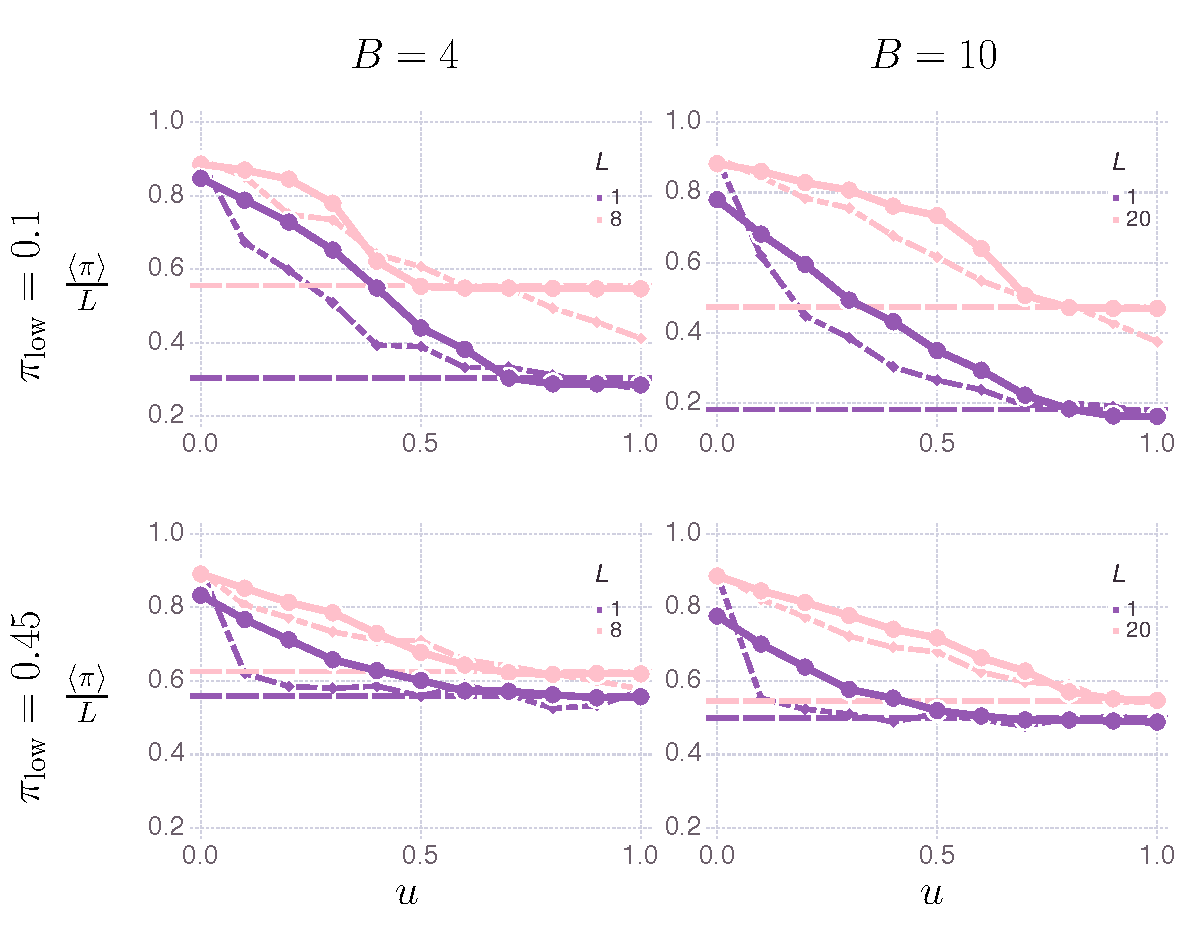
\includegraphics[width=0.85\textwidth]{Figures/meanNetPayoffs.pdf}
\end{figure}

We confirmed that drift increased when $\meansl$ transitioned from 1 to 0, 
and when $\pilow$ was increased. We measured drift by the average number of 
generations to fixation, $\meanG$. Recall fixation is defined as the population
becoming homogenous, composed of all social or all asocial learners. 
$\meanG$ peaks around the values of $u$ 
when $\meansoc \approx \meanasoc$, which led $\meansl$ to transition from 1 to 0.
In some cases, especially when $\pilow=0.8$,
there is no distinct peak in $\meanG$ across $B$ and $L$ settings, 
indicating little difference in task difficulty across a range of uncertainty parameter settings.


\begin{figure}
  \caption{Average number of generations ($\meanG$, y-axes) to fixation . 
    $\meanG$ increases and peaks around values of $u$ (x-axes) where
  $\meansoc \approx \meanasoc$. Note the y-axis ticks vary between plots,
indicating different overall time to fixation for different $(\pilow, B)$
pairs. Only extremal tested values of $L$ shown for clarity.} 
  \label{fig:steps}
\centering
    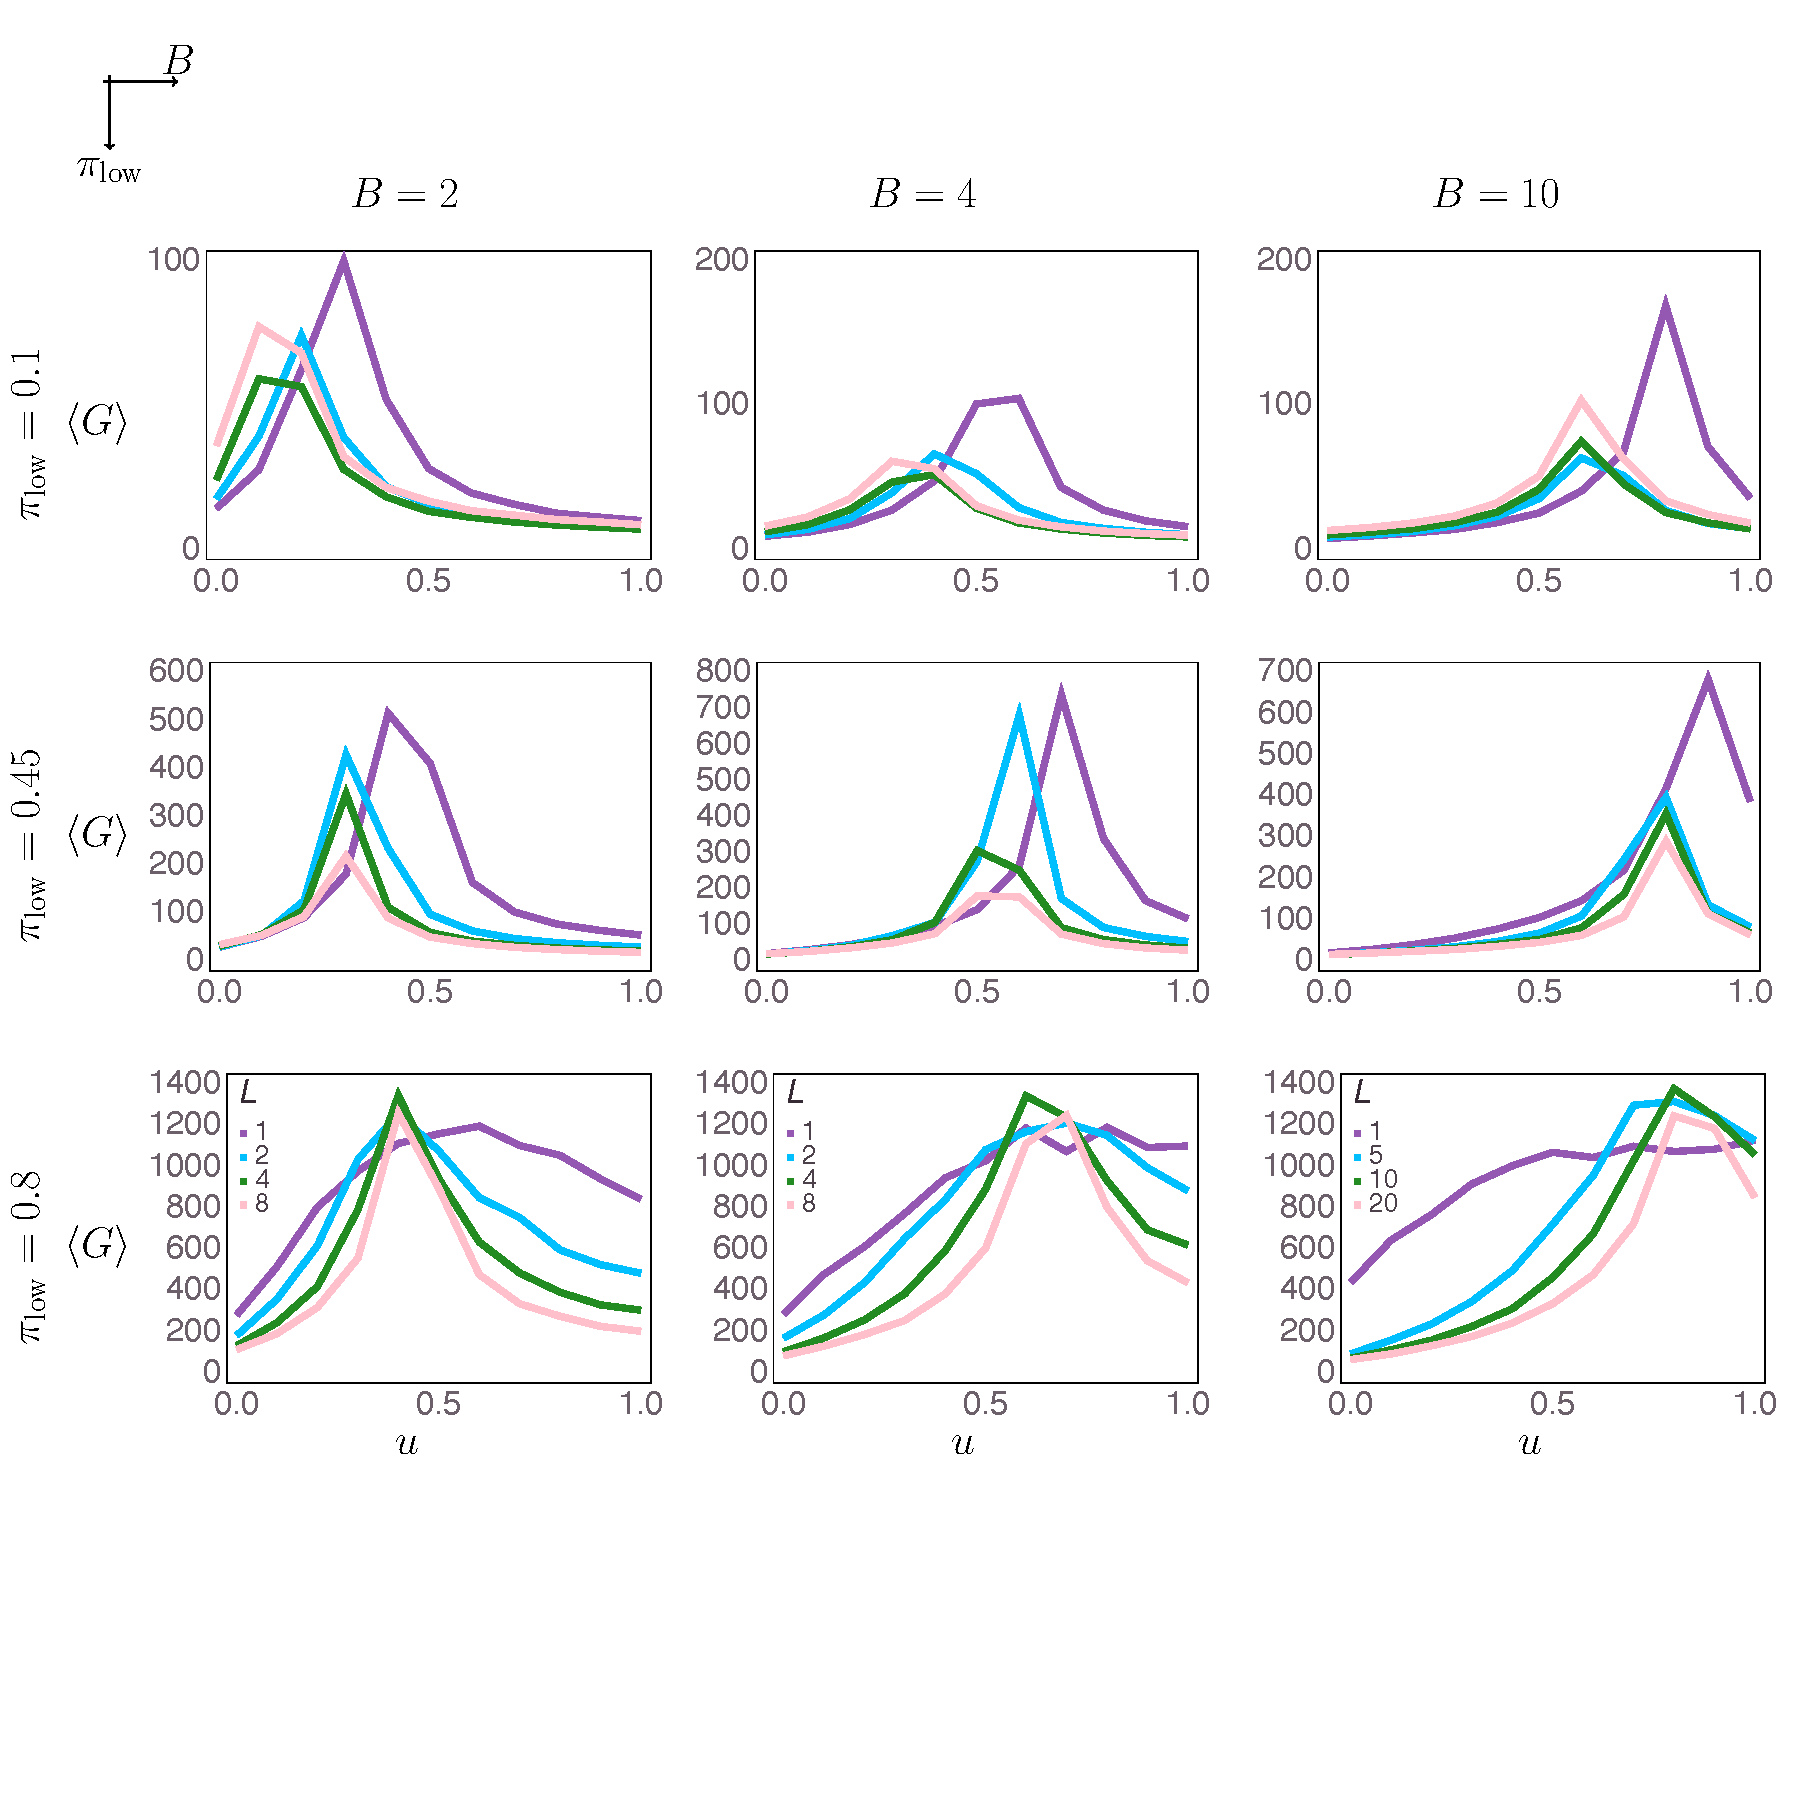
\includegraphics[width=\textwidth]{Figures/stepResultsPlots.pdf}
\end{figure}



\section{Discussion}



By disambiguating and organizing various operationalizations of
uncertainty, we developed a more nuanced theoretical understanding of which forms of
uncertainty interact to affect social learning.  We reviewed and distilled the several empirical and
theoretical models in the literature along four uncertainty dimensions: temporal
environmental uncertainty, selection set size, ambiguous payoffs, and effective lifespan.
The model reproduced classic predictions that social learning can yield higher payoffs
than individual learning when uncertainty is sufficiently limited. Our model also
demonstrated a new insight into social learning as a scaffold for individual learning,
enabled by endowing agents with an evolutionarily- and biologically-plausible individual
learning mechanism, softmax search. Specifically, we found that agents could recover from
receiving outdated information, so social learning could evolve even though social
information was outdated more often than not. We found increased payoff ambiguity and
lifespan led to greater drift, which is essentially evolutionary uncertainty in a
finite-size population. Detailed theoretical models and
predictions of cultural evolution under uncertainty are critical for understanding how
humans adapt to an uncertain and rapidly changing world, both to mitigate existential
threats~\cite{Moya2020,Jones2021}, especially in the most vulnerable
communities~\cite{McNamara2020}, and to capitalize on new behavioral opportunities such as
transitioning to clean energy use and
production~\cite{NatureEnergyEditorialPromisesPremises2018,Brisbois2022}.

Our modeling choices were judiciously made to address the main question of how uncertainty
affects the evolution of social learning in general; however there exist alternative
empirically-valid choices that could help further develop a more nuanced theory of social
learning.  Our model necessarily made simplifying assumptions that may not always hold in more
specific situations, though they are empirically justified to be general across taxa. First,
note that we only considered success-biased learning, although conformity is sometimes the
dominant social learning mechanism~\cite{Muthukrishna2016a,Smaldino2018b}.  Conformity may lead
to more drift overall, since success-biased teacher selection, which we assumed, maximizes the
potential benefit to social learners. We assumed that the number of behaviors and their payoffs
were constant, but this fails to account for evolutionary feedback which creates new behavioral
opportunities as time progresses, e.g.\ via niche
construction~\cite{Smaldino2012a,Heras-Escribano2020} or cumulative cultural evolution
supported by dynamic network structure~\cite{Smolla2019,Derex2020}.  Group structure and
processes such as homophily and in-group bias/out-group aversion could inhibit the evolution of
social learning since successful outgroup teachers could be cut off from in-group
learners~\cite{Jackson2012}. We assumed agents choose behaviors via softmax search, but this is
an underpowered algorithm compared to human individual learning~\cite{Schulz2020a,Wu2022}.
More powerful individual learning could further support social learning.  These considerations
reveal new opportunities to further by adjusting or extending the present model for other
contexts. 


\subsection{Conclusion}

We found that the evolution of social learning, under a few modest assumptions, is a
complex phenomenon, dependent on several interrelated factors. By systematically
identifying and operationalizing common theoretical assumptions about contextual
uncertainty in social learning models, we were able to develop a more systematic
understanding of which uncertainty factors interact to determine whether social learning
evolves. By explicitly modeling a key individual-level learning mechanism shared across taxa, namely the
ability to adjust behavior to uncertainty and new information, we saw that social
learning could evolve even if social learning regularly provides outdated
information. This work informs most directly our current understanding of the evolution of
social learning, but has broader significance for understanding problem
solving under uncertainty. Our model and its software implementation were
designed to be modular and extensible.  Indeed, we plan to extend this model to further
develop a more detailed theoretical understanding of the evolution of social learning;
we hope others will, too.


\bibliographystyle{apacite}
% \bibliography{/Users/mt/workspace/Writing/library.bib}
\bibliography{this.bib}


\appendix


\section{Appendix}

\mt{TODO: Write supporting material explaining supplemental results}

\subsection{Convergence information}

\mt{These here used $N=100$; need to remake with $N=1000$}

\begin{table}[h] \caption{Max. iterations = 20000.} \label{tab:convergence} \centering
  \begin{tabular}{cccc} \toprule $B$ & \# not at fixation & \# total series & Pct. not fixated
    \\ \midrule  2  & 0  & 132000 & 0.0 \% \\ 4  & 0  & 132000 & 0.0 \% \\ 10 & 44 & 132000 &
    0.00033  \% \\ \bottomrule \end{tabular} \end{table}


\newpage

\subsection{Full net payoff comparison for all nine uncertainty conditions} 

\begin{figure}
  % \addtocounter{figure}{-1}
  \caption{Comparison of expected payoffs from our computational anaysis (solid
    lines with circles), expected individual payoffs with no social learning
    (dashes without markers), and expected payoffs for all-social learner 
    populations. When $\pilow = 0.8$, all-social learner populations underperform
    since social learners are not subject to an initial evolutionary bottleneck
    due to the presence of asocial learners, and behavioral misinformation
    is allowed to circulate more freely than in the base case tested by 
    our model with an initially even distribution of social and asocial learners.
}
  \label{fig:fullMeanPrevNetPayoffs}
  \centering
    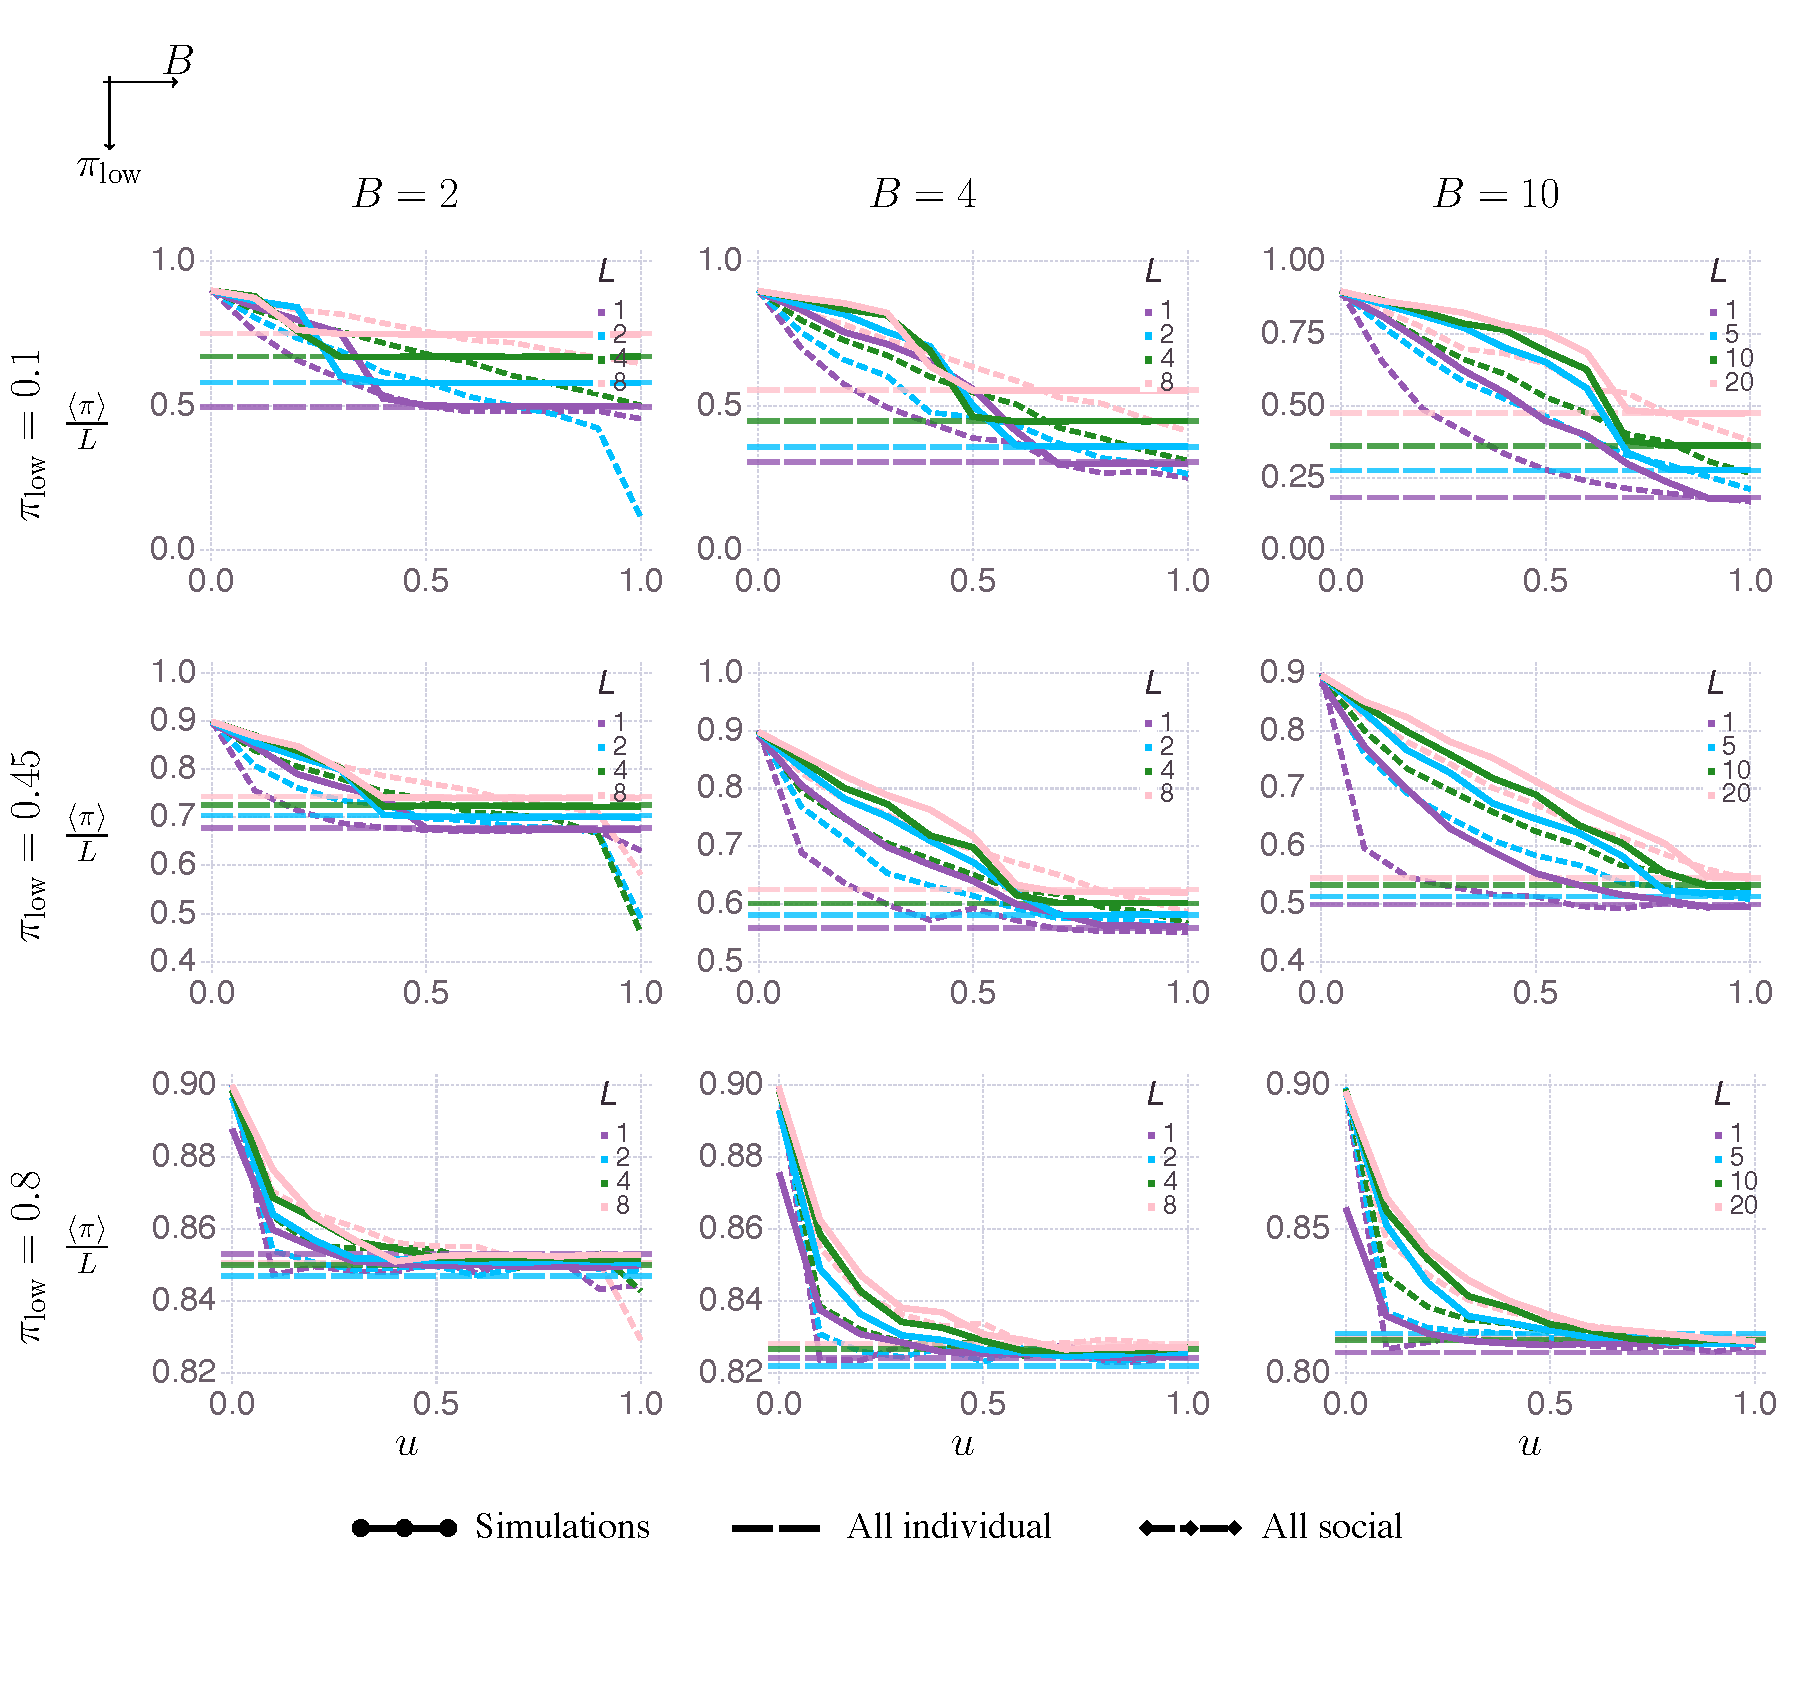
\includegraphics[width=\textwidth]{Figures/supplement/fullMeanPrevNetPayoffs.pdf}
\end{figure}



\subsection{Softmax parameter sensitivity analysis} 

\mt{These here used $N=100$; need to remake with $N=1000$}

\vspace{-3em} \begin{figure} %\addtocounter{figure}{-1} 
  \centering
  \caption{Sensitivity analysis of the main results for the softmax parameter $\beta = 100$ and
  $\beta=1$. Recall the main results were obtained with $\beta = 10$.}
  \label{fig:softmaxSensitivity} \vspace{2em}
  \begin{subfigure}{\textwidth}
	\caption{$\beta = 100$}
	\includegraphics[width=\textwidth]{Figures/supplement/sensitivity_tau=0.01/mainResultsPlots.pdf}
  \end{subfigure}
\end{figure}
\newpage
\begin{figure}
  \ContinuedFloat
  \begin{subfigure}{\textwidth}
	\caption{$\beta = 1$}
	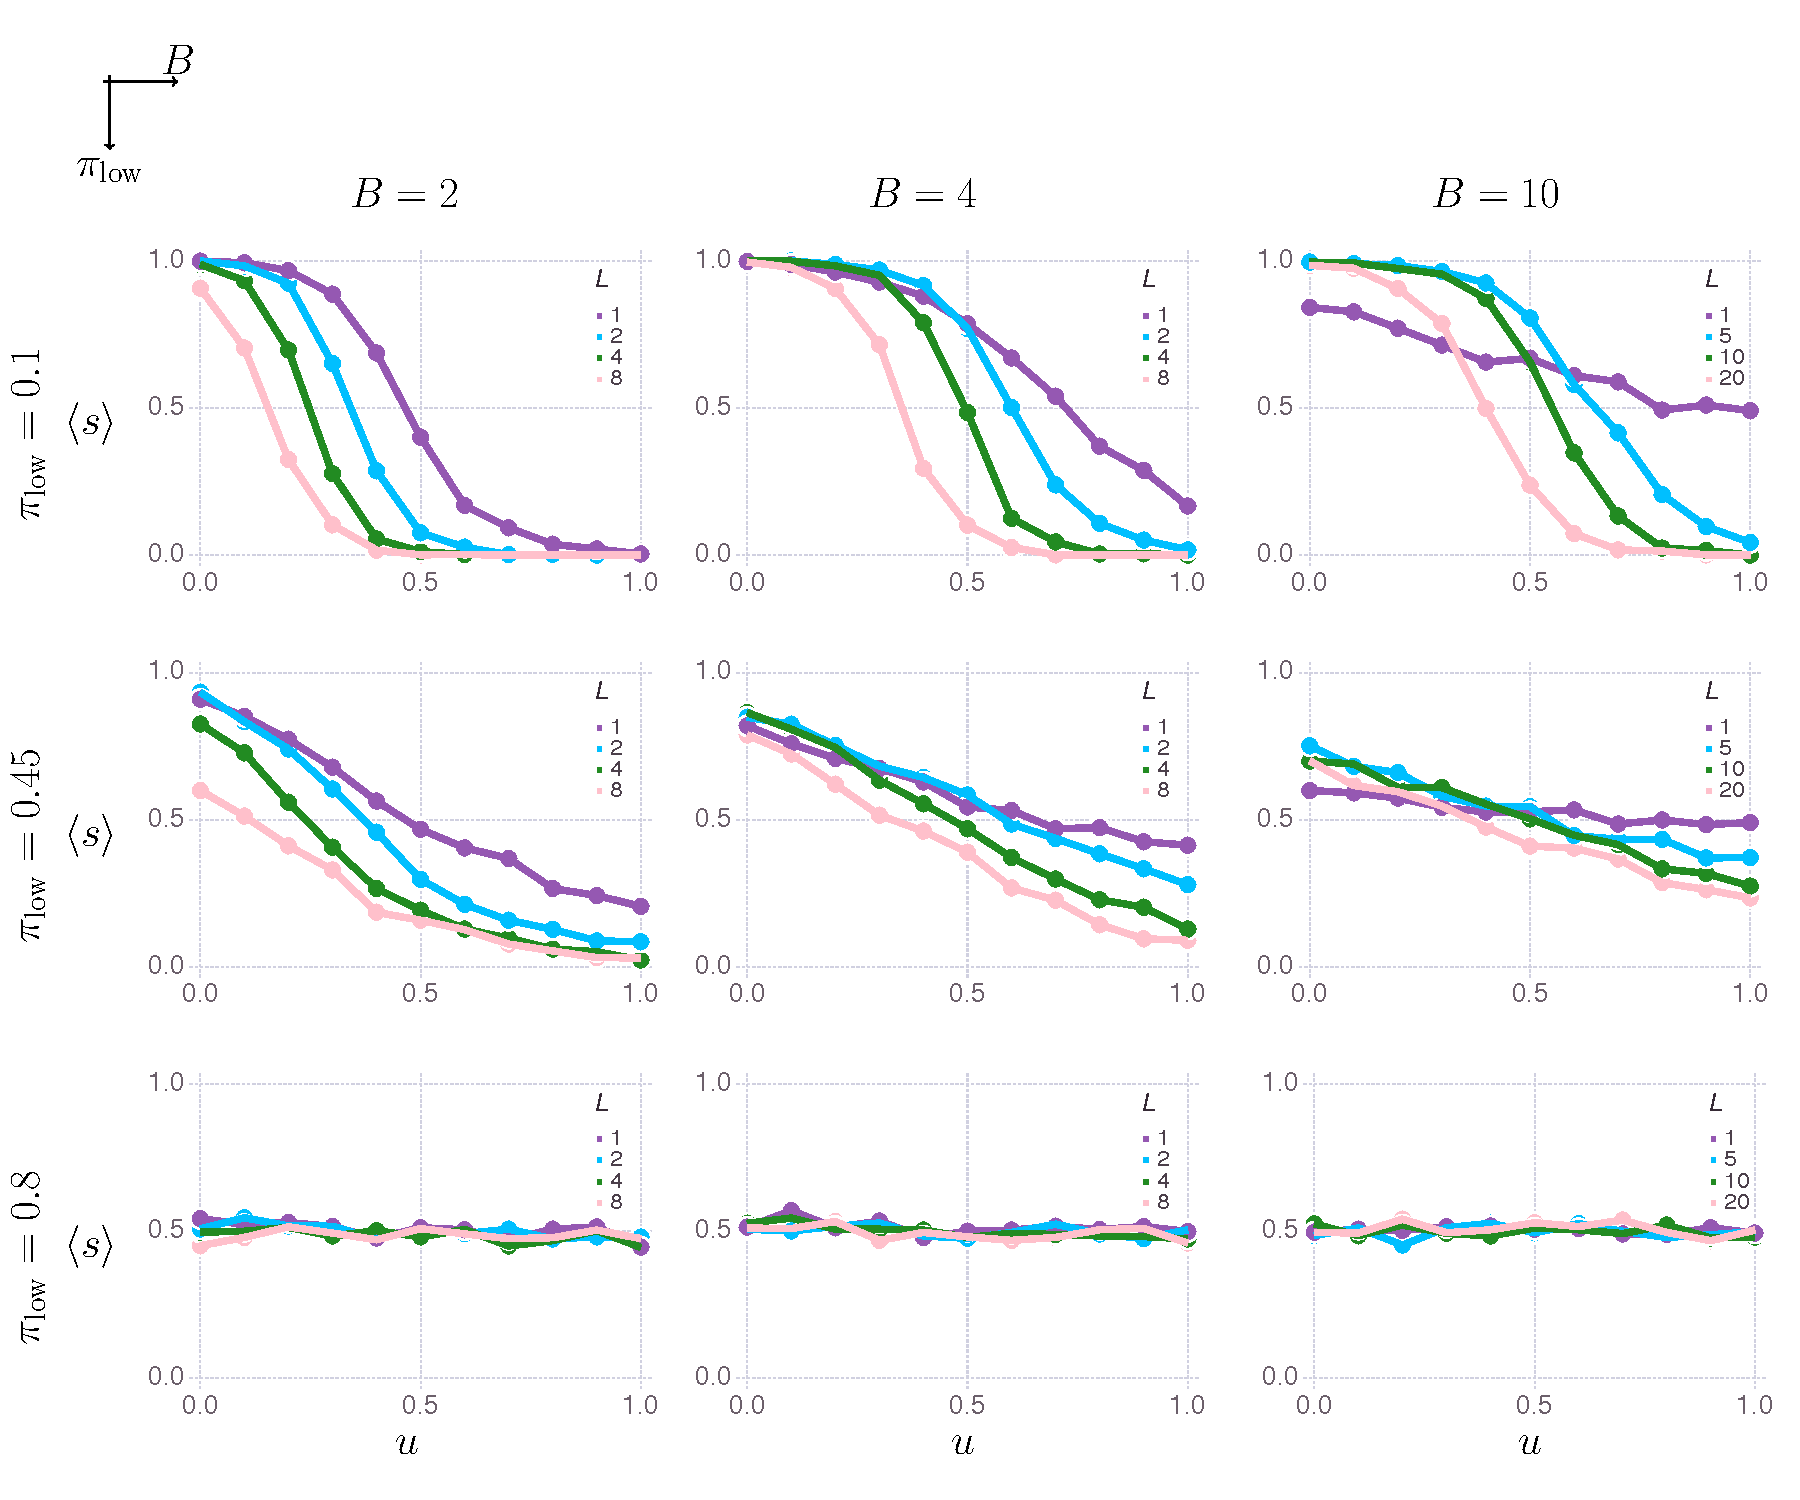
\includegraphics[width=\textwidth]{Figures/supplement/sensitivity_tau=1.0/mainResultsPlots.pdf}
  \end{subfigure}
\end{figure}


\newpage
\subsection{Population size sensitivty analysis}

\begin{figure}
  \centering
  \caption{
	Sensitivity analysis of the main results for different population
	sizes, $N=50,200,1000$. Recall $N=100$ was used to generate main 
	text results.
  }
  \label{fig:populationSensitivity}
  \begin{subfigure}{\textwidth}
	\caption{$N=50$}
	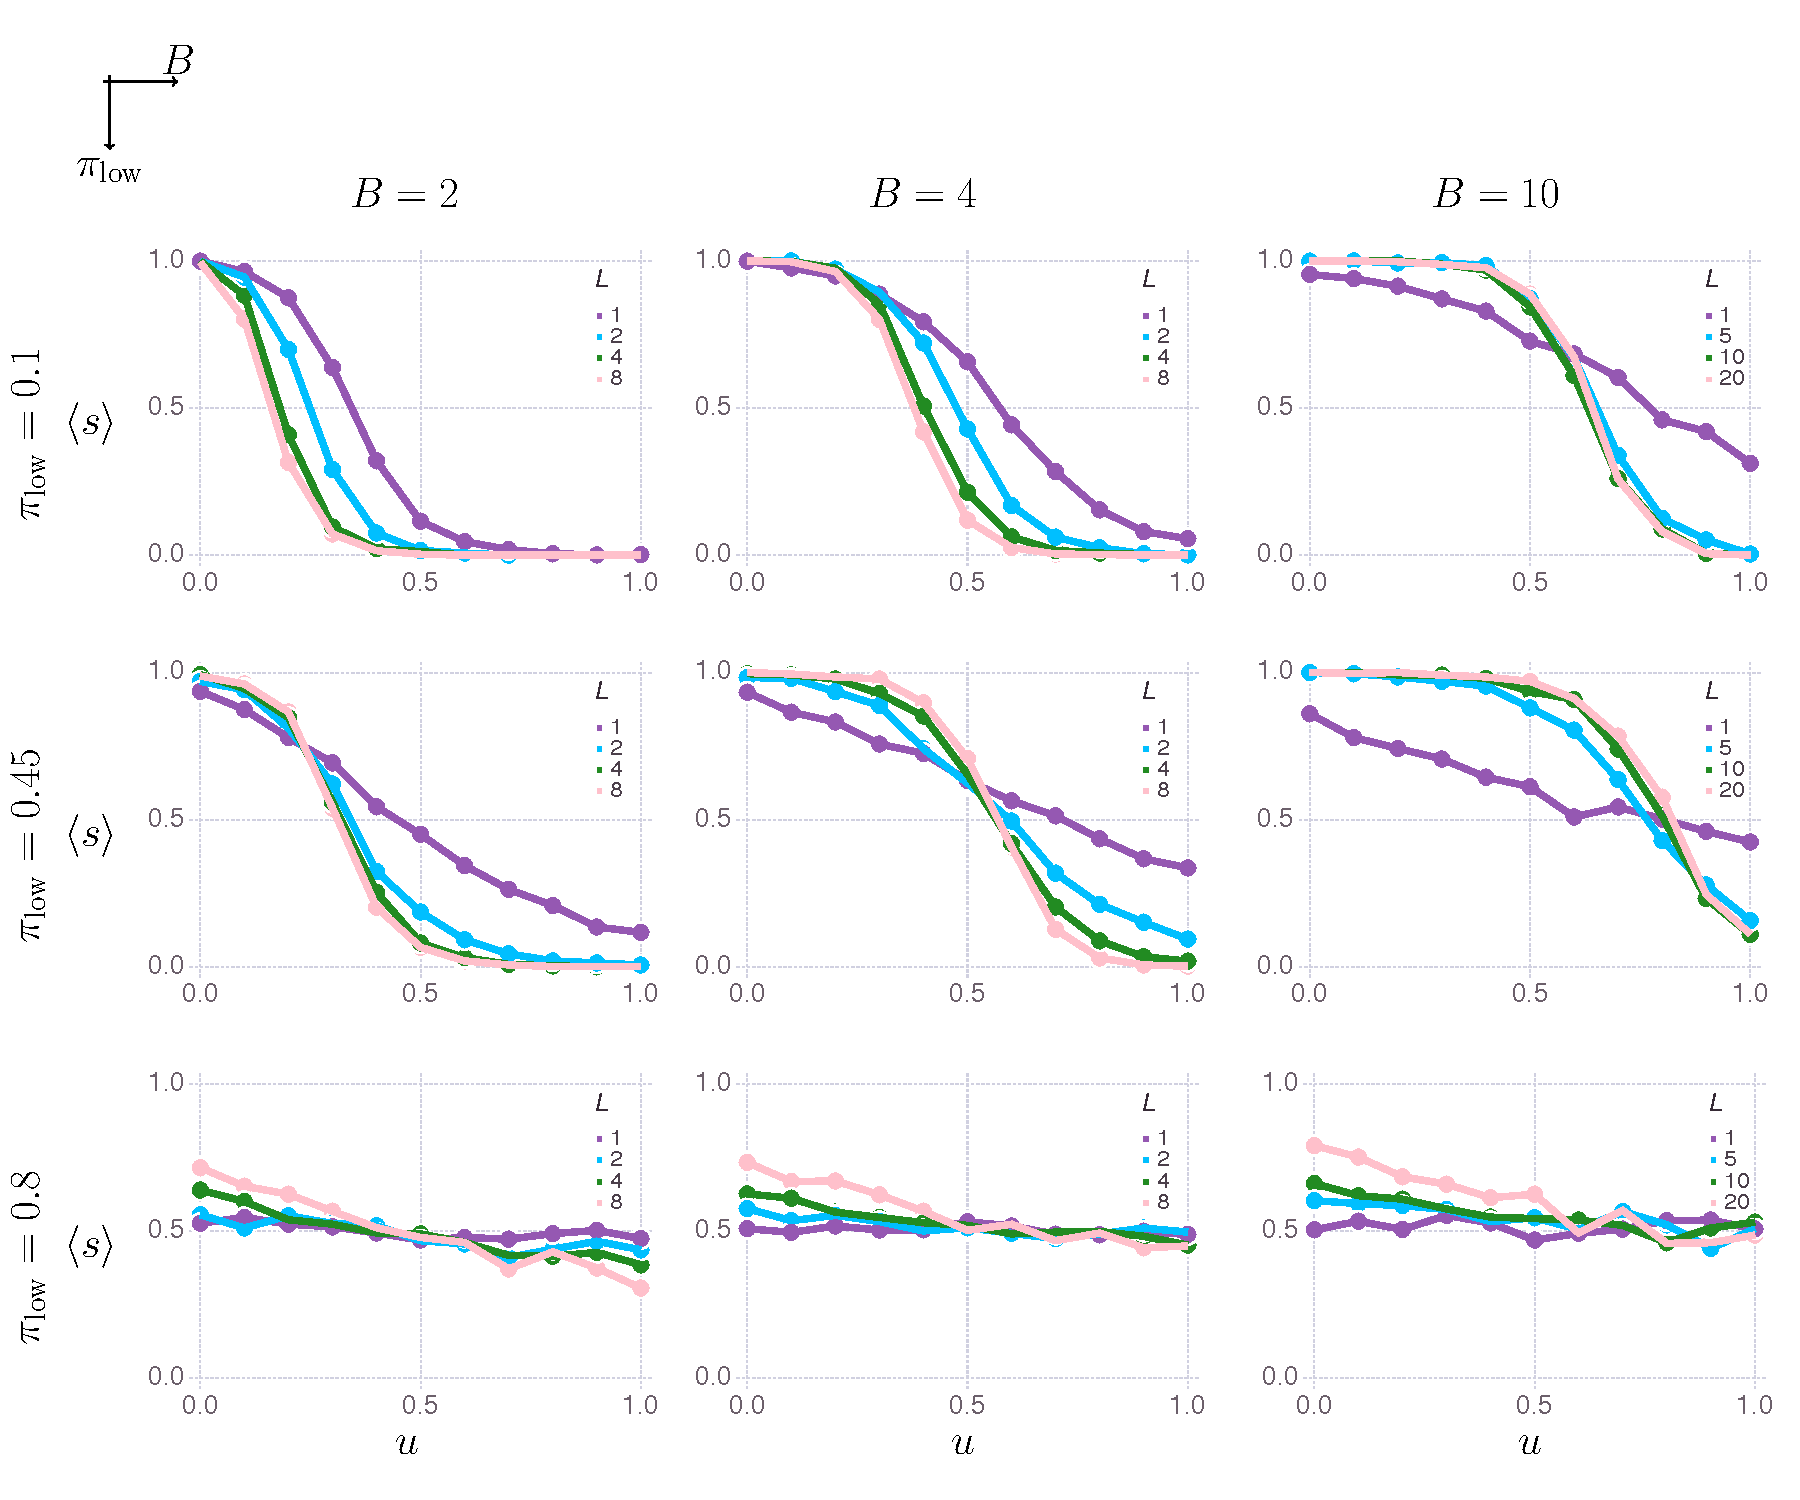
\includegraphics[width=\textwidth]{Figures/supplement/nagents=50/mainResultsPlots.pdf}
  \end{subfigure}
\end{figure}

\begin{figure}
  \ContinuedFloat
	\begin{subfigure}{\textwidth}
	  \caption{$N=100$}
	  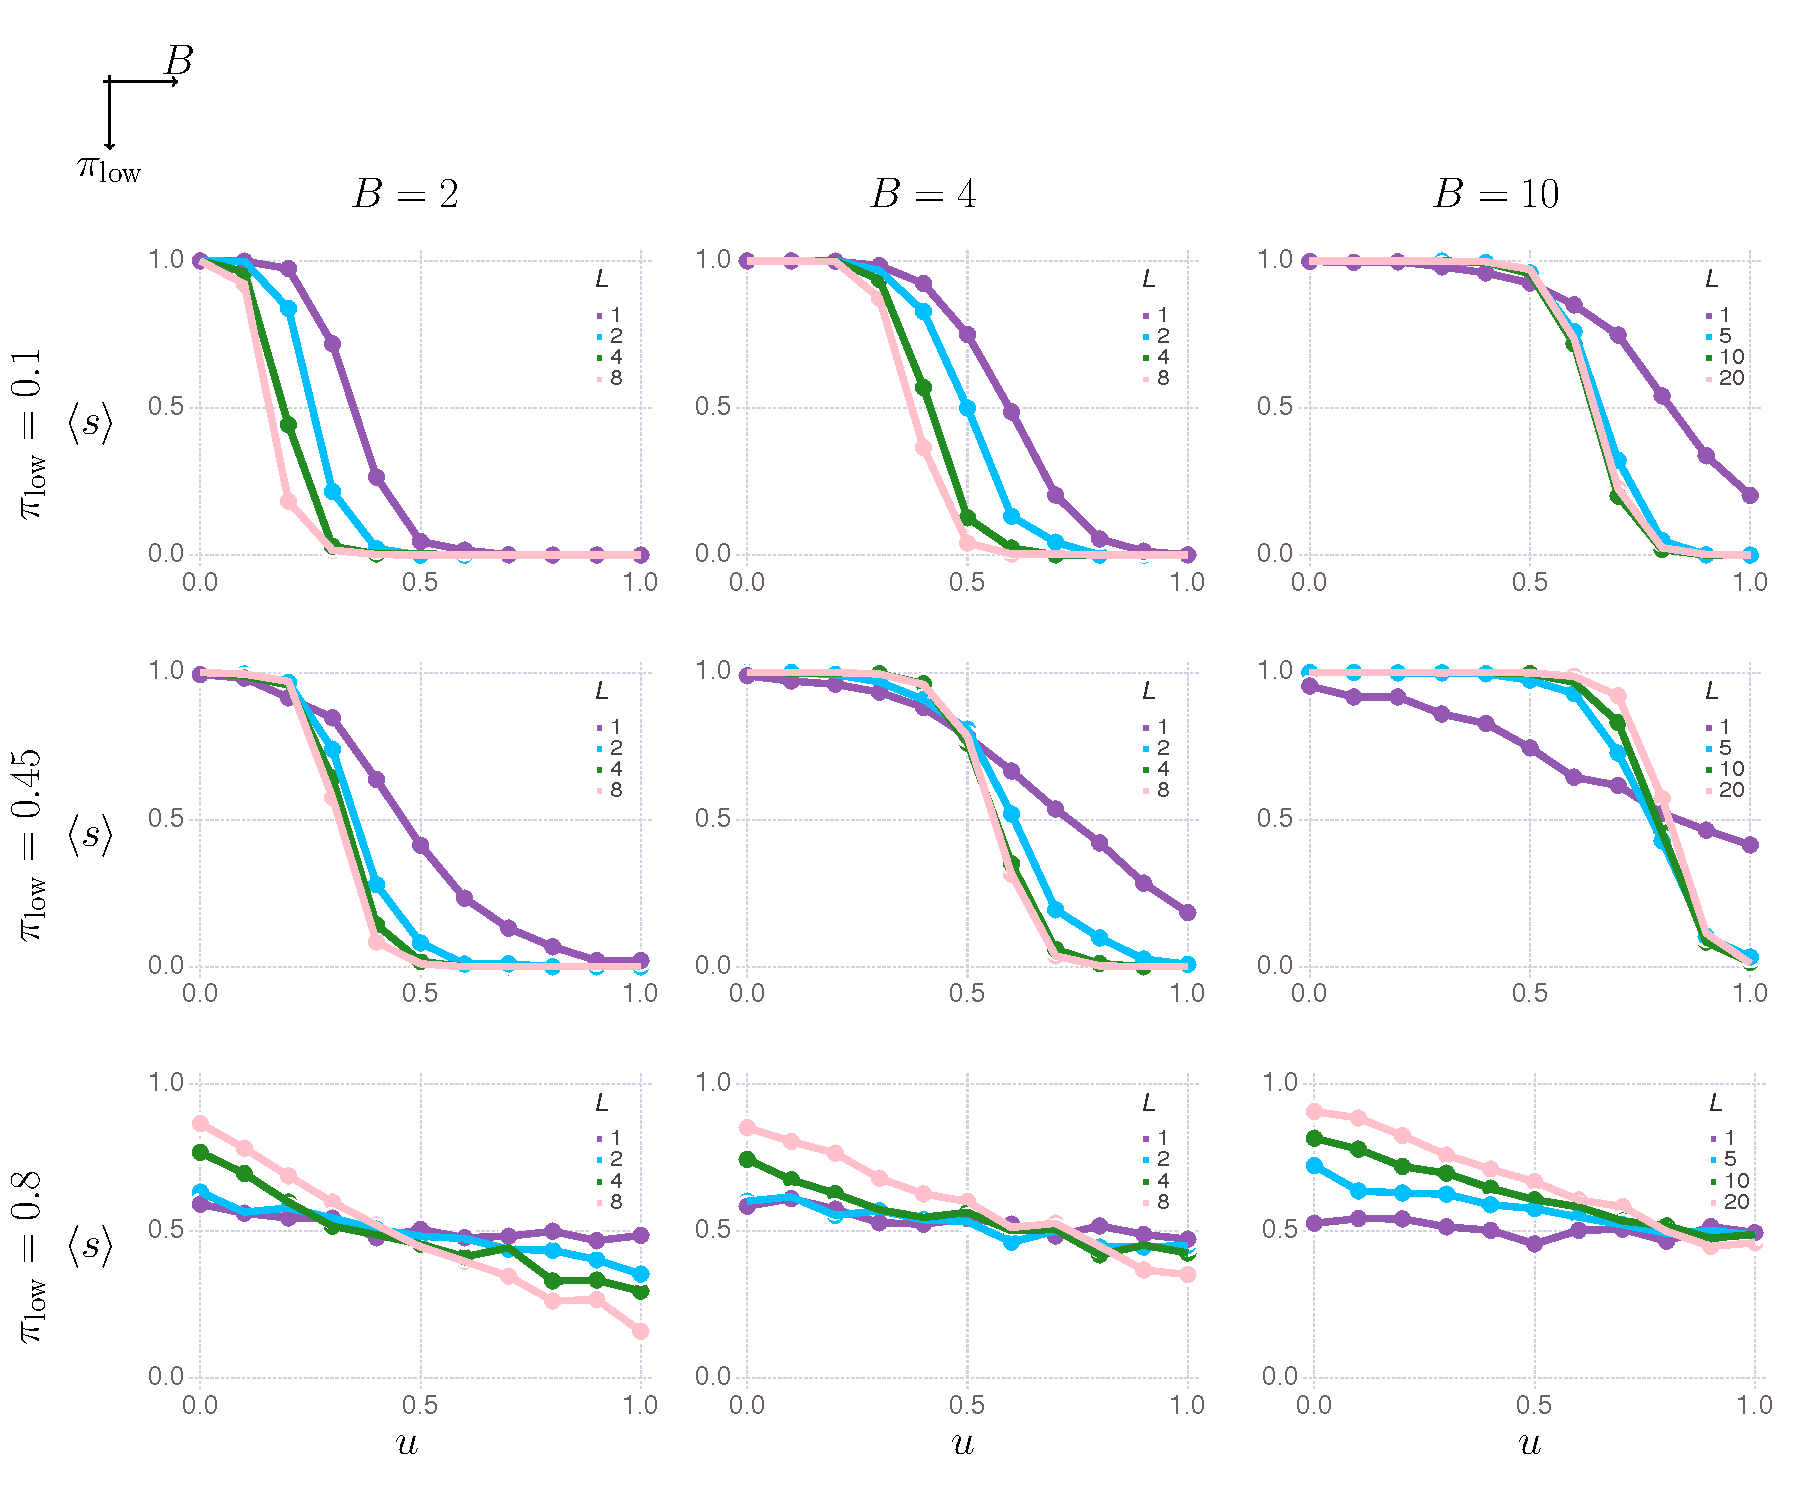
\includegraphics[width=\textwidth]{Figures/mainResultsPlots.pdf}
	\end{subfigure}
\end{figure}
	
\begin{figure}
  \ContinuedFloat
	\begin{subfigure}{\textwidth}
	  \caption{$N=200$}
	  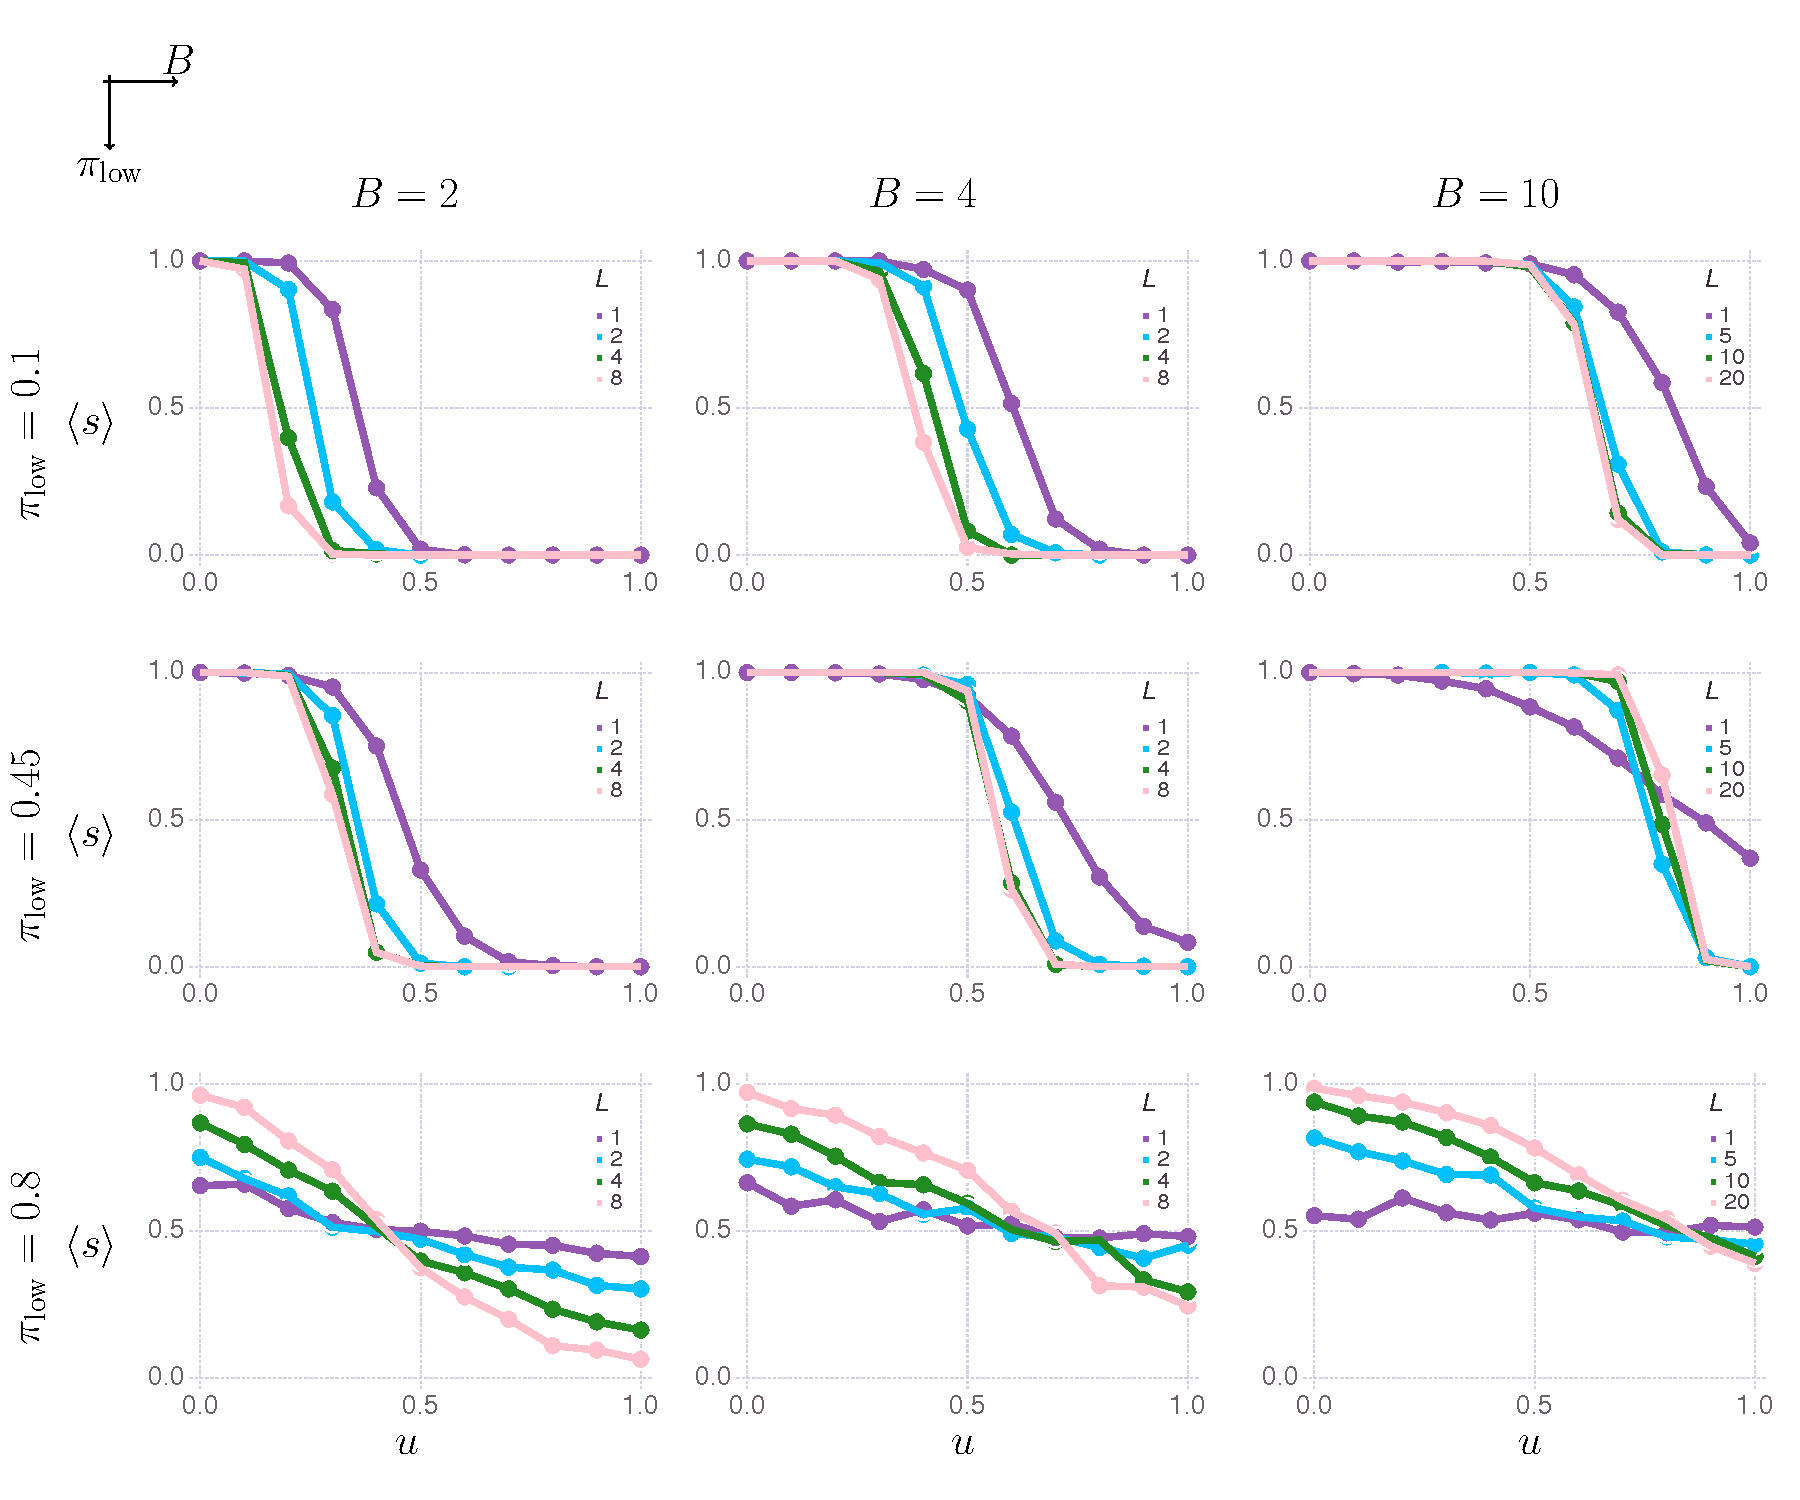
\includegraphics[width=\textwidth]{Figures/supplement/nagents=200/mainResultsPlots.pdf}
	\end{subfigure}
\end{figure}


\newpage
\subsection{Number of prospective teachers sensitivty analysis}

\mt{These here used $N=100$; need to remake with $N=1000$}

\vspace{-3em}
\begin{figure}
  \centering
  \caption{Number of prospective teachers sensitivity analysis for $N_T=2,10,20$. Recall
  $N_T=5$ was used to generate main text results.}
  \label{fig:softmaxSensitivity}
  \vspace{2em}
  \begin{subfigure}{\textwidth}
	\caption{$N_T = 2$}
	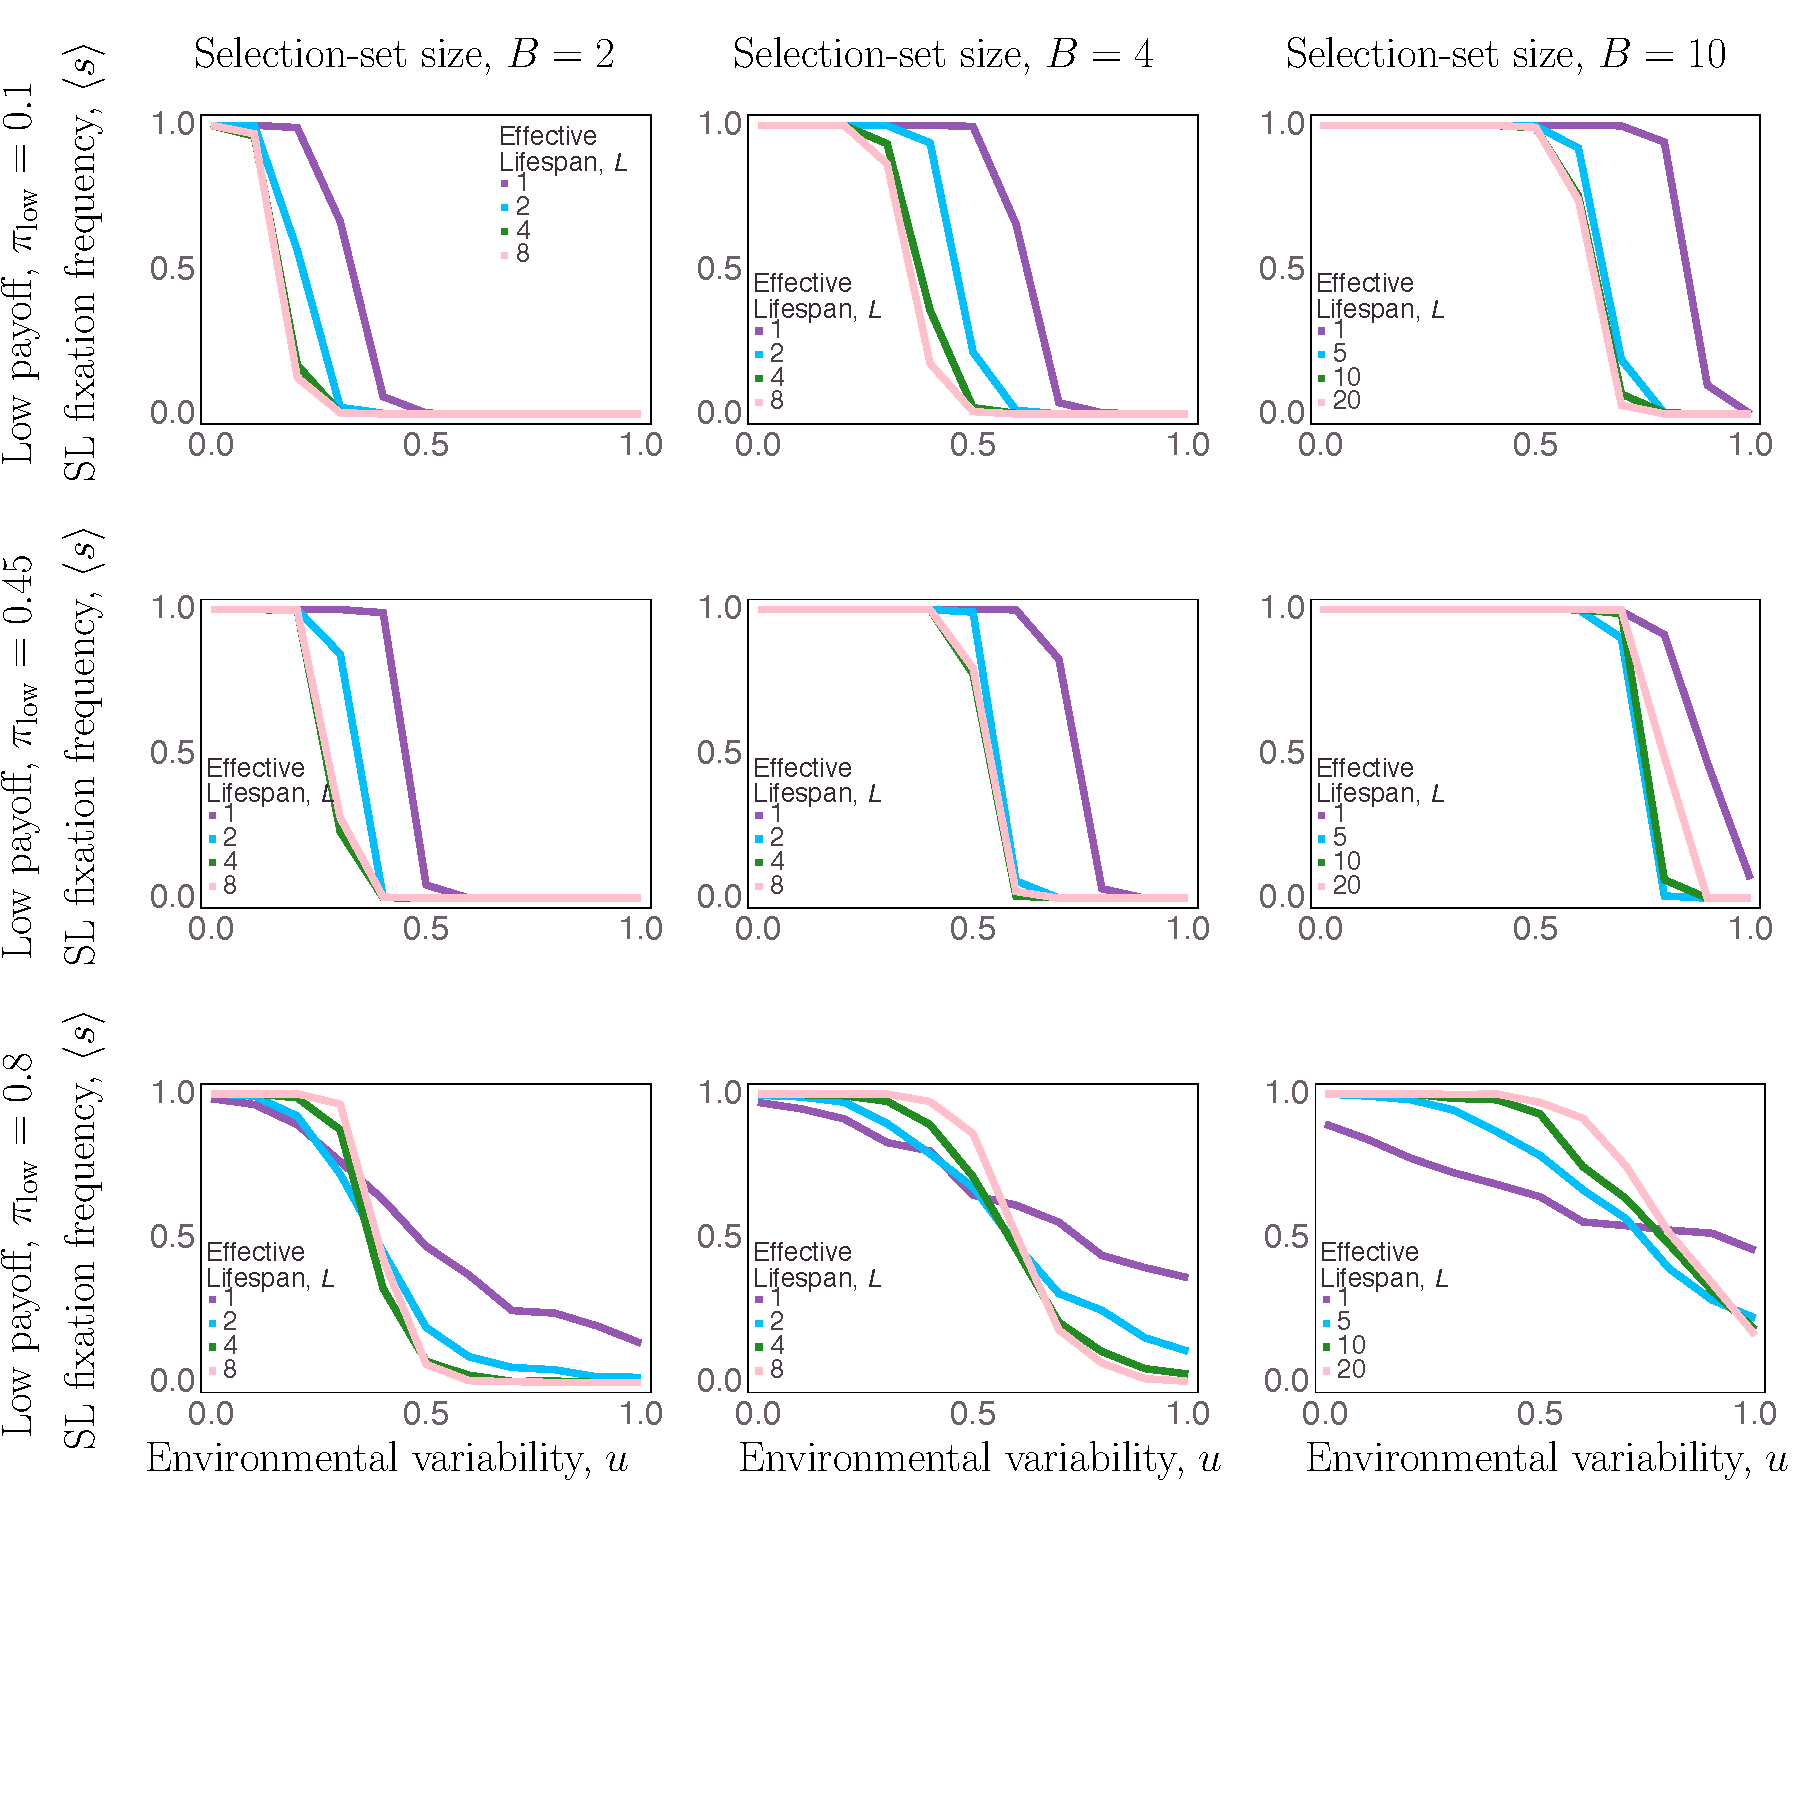
\includegraphics[width=\textwidth]{Figures/supplement/nteachers=2/mainResultsPlots.pdf}
  \end{subfigure}
\end{figure}
\newpage
\begin{figure}
  \ContinuedFloat
  \begin{subfigure}{\textwidth}
	\caption{$N_T = 10$}
	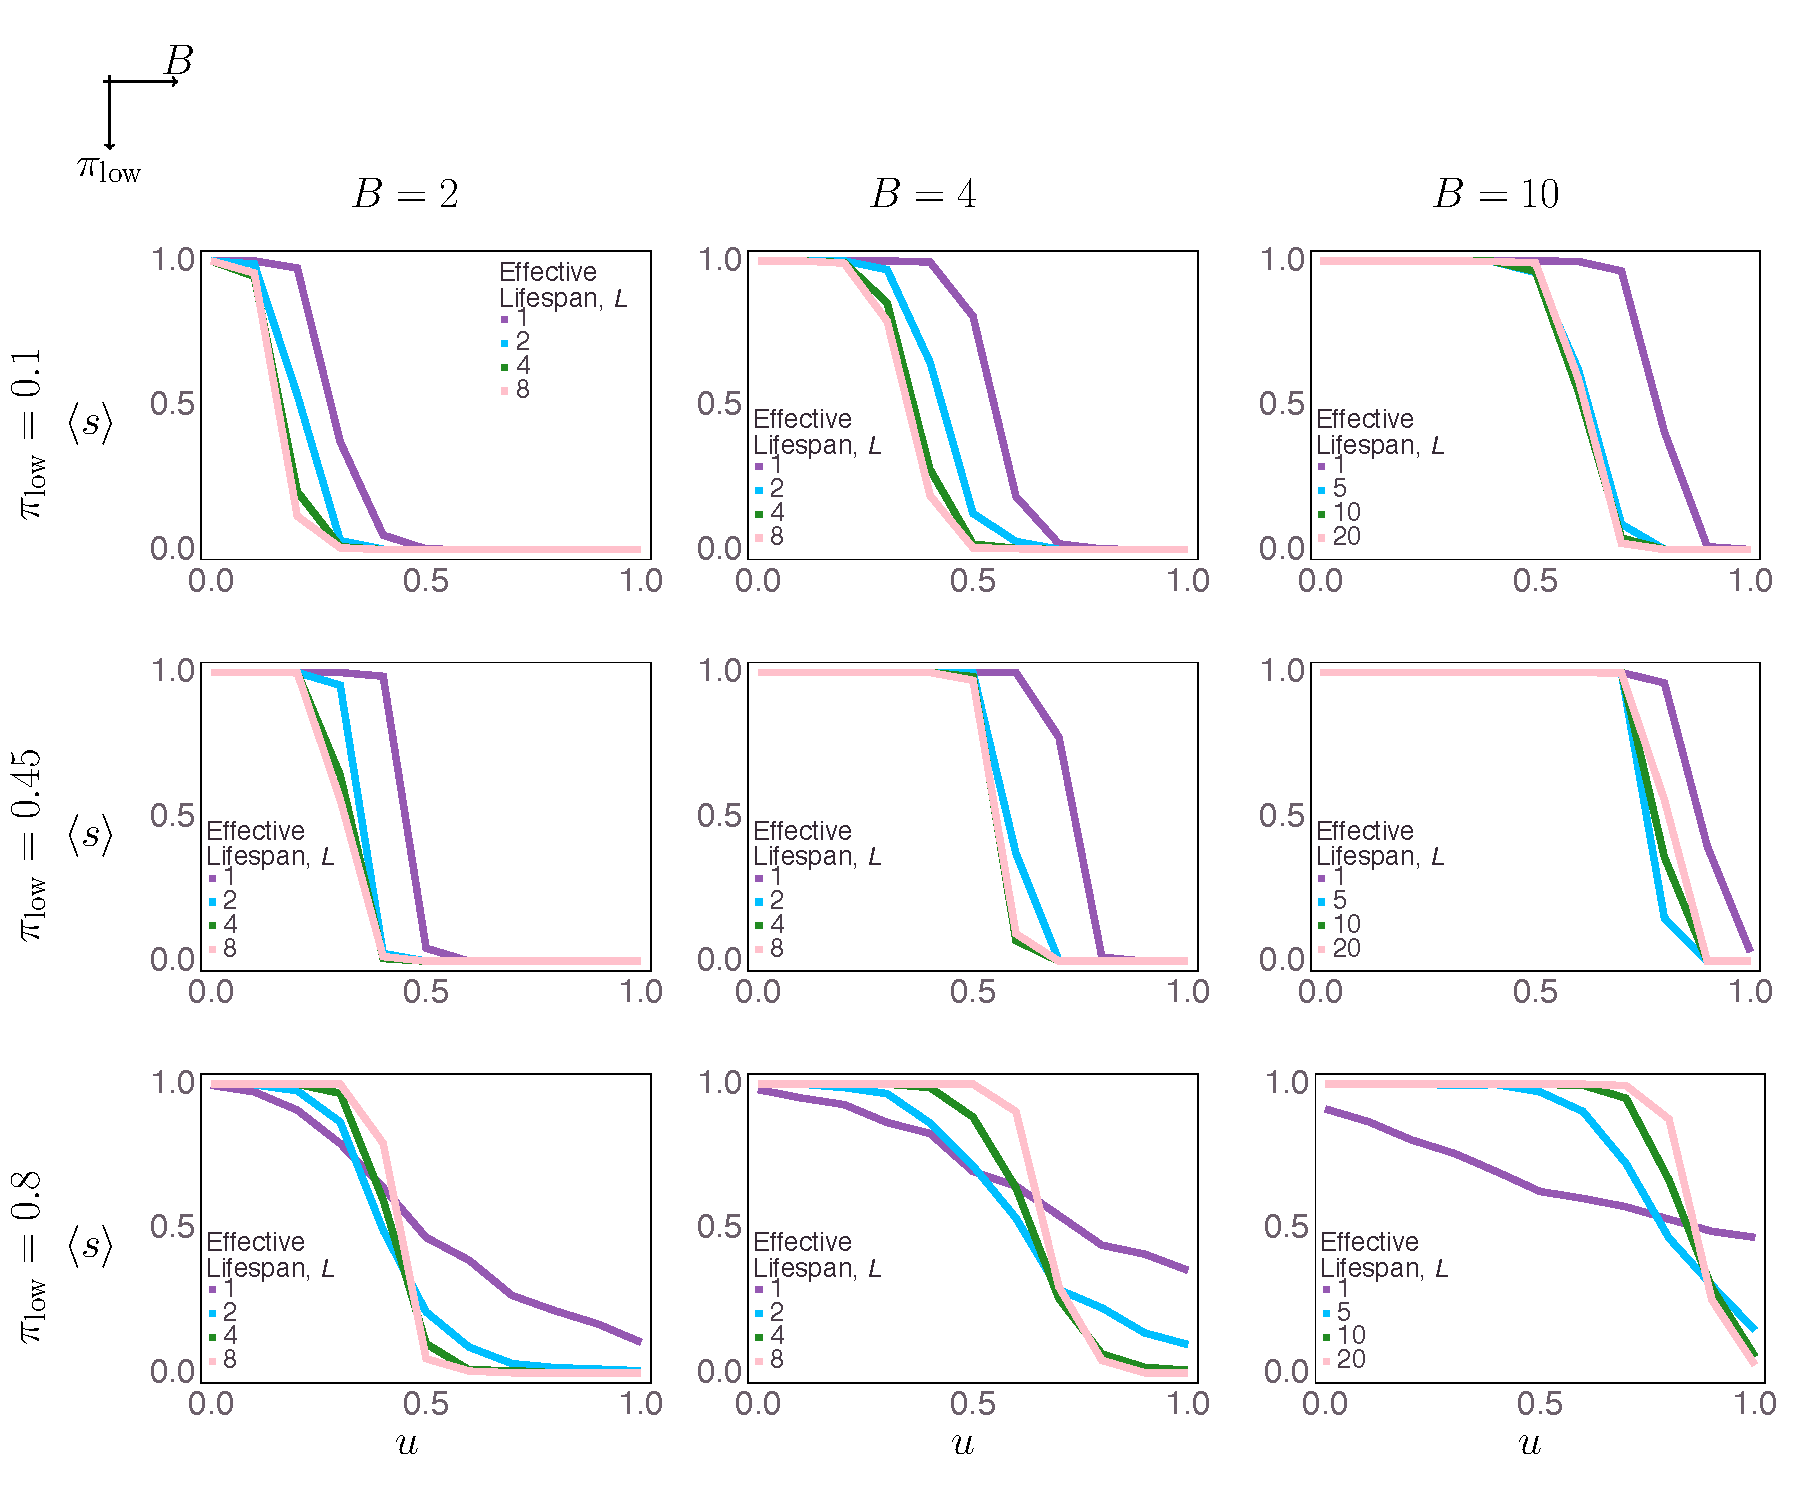
\includegraphics[width=\textwidth]{Figures/supplement/nteachers=10/mainResultsPlots.pdf}
  \end{subfigure}
\end{figure}
\newpage
\begin{figure}
  \ContinuedFloat
  \begin{subfigure}{\textwidth}
	\caption{$N_T = 20$}
	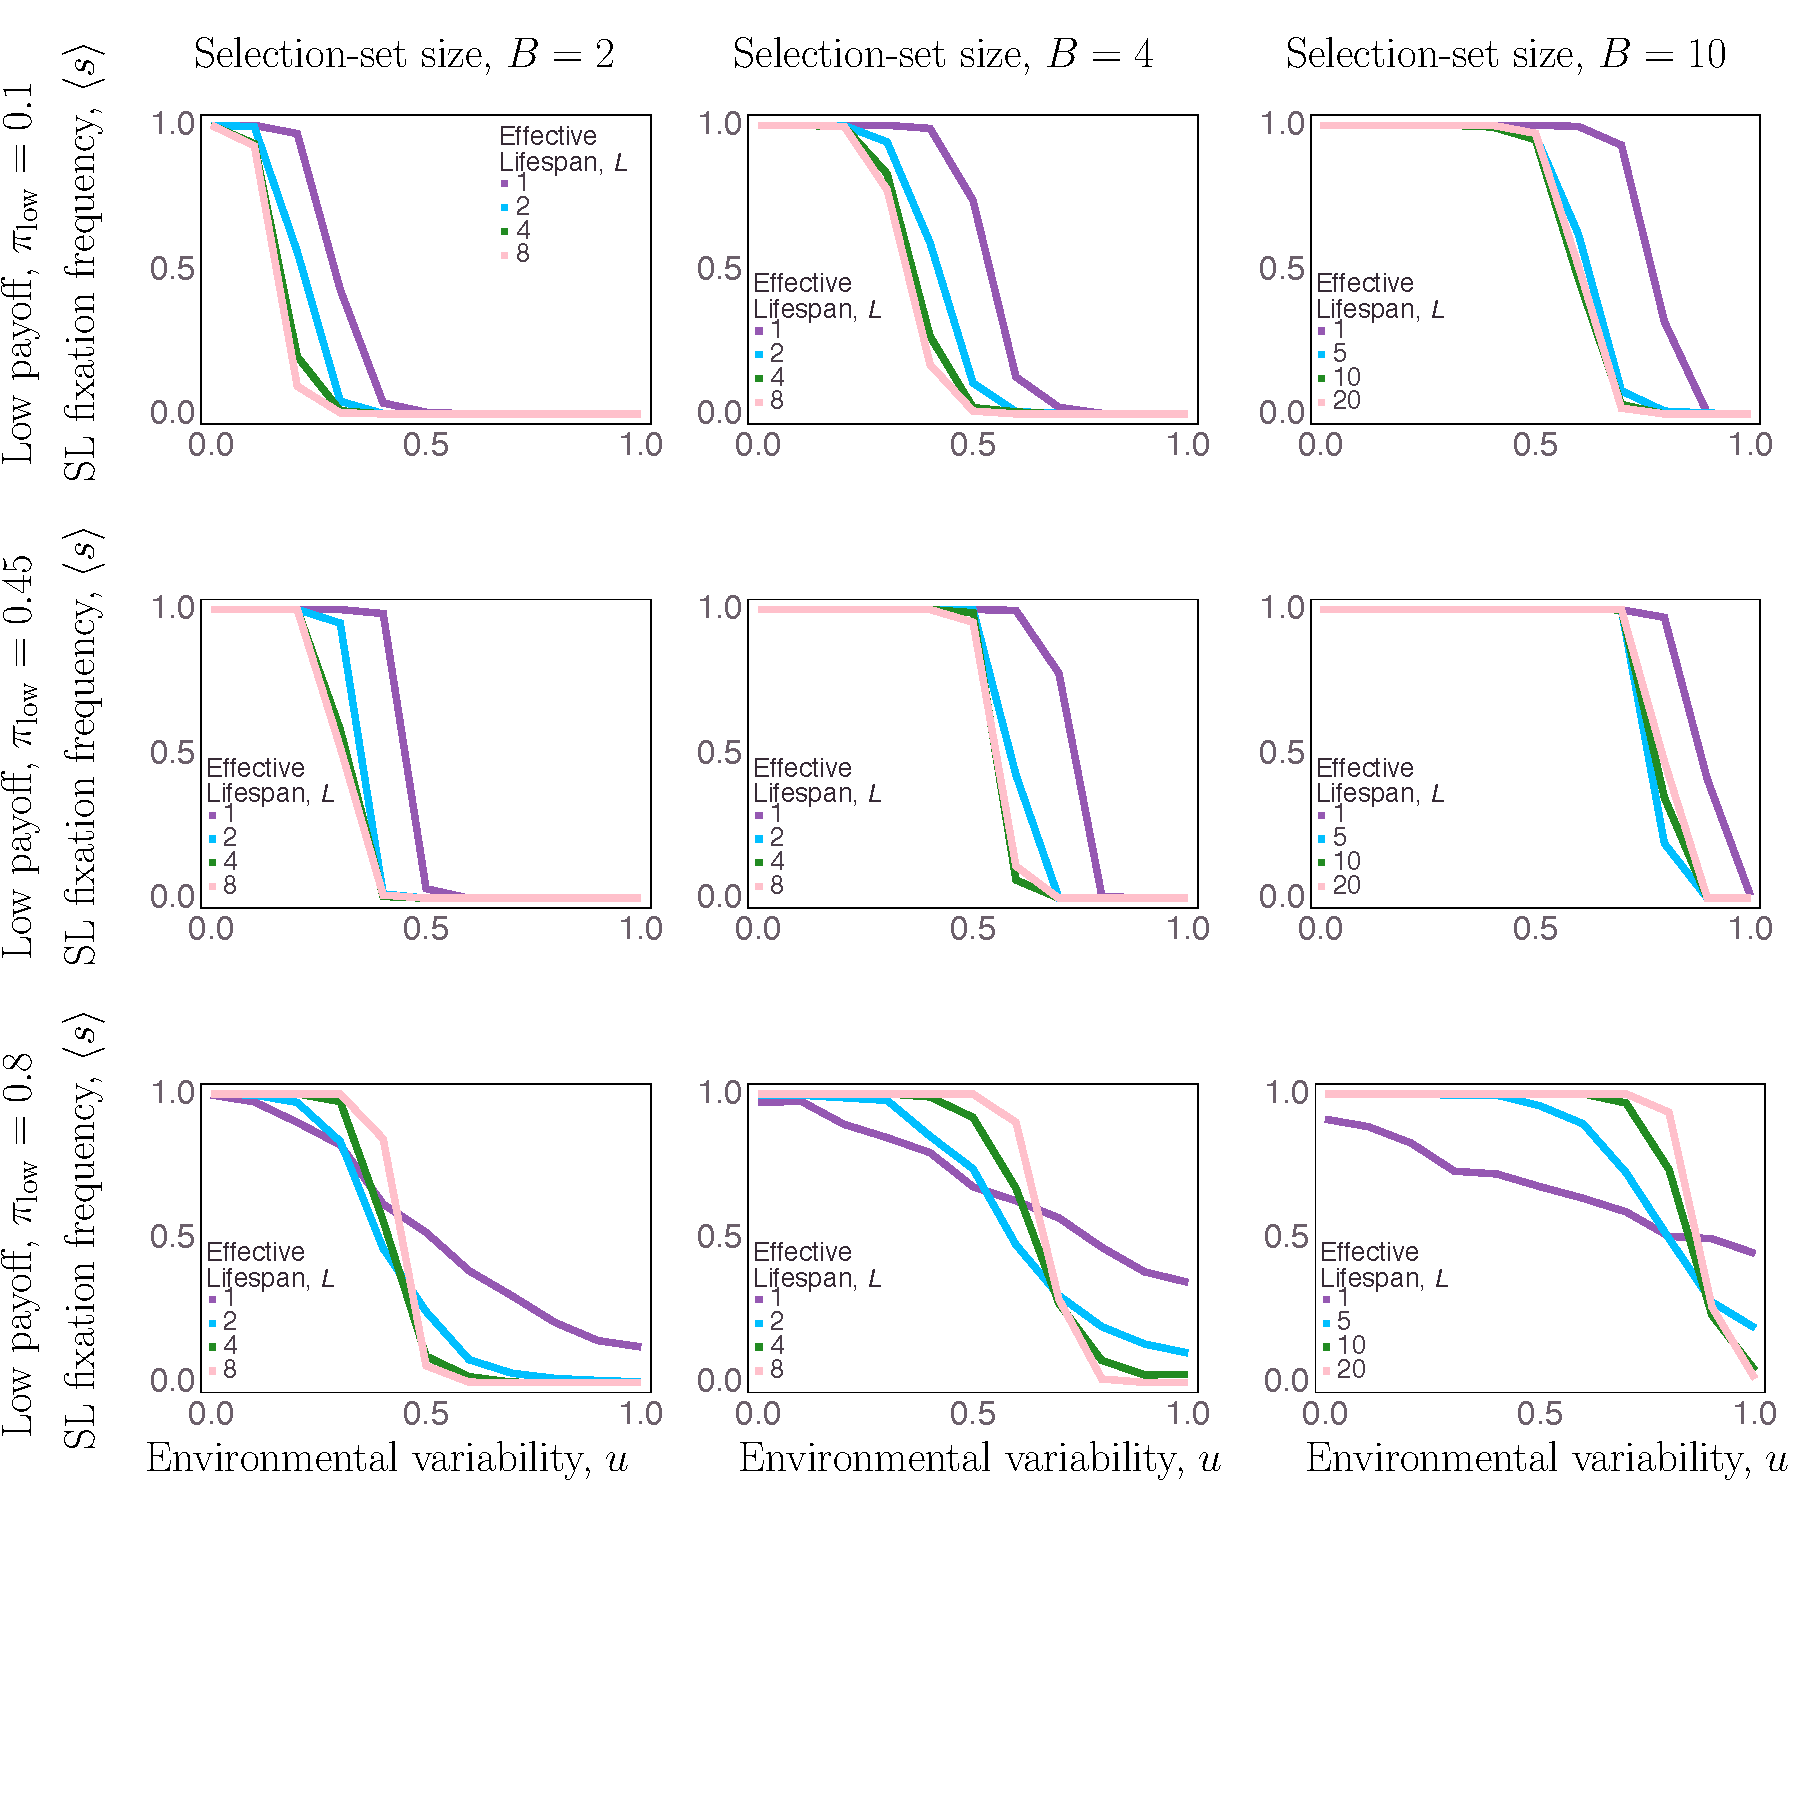
\includegraphics[width=\textwidth]{Figures/supplement/nteachers=20/mainResultsPlots.pdf}
  \end{subfigure}
\end{figure}


\end{document}
